\section{昇腾310B开发板介绍}\label{ux6607ux817e310bux5f00ux53d1ux677fux4ecbux7ecd}

OrangePi
AIpro(8T)开发板是香橙派联合华为精心打造的高性能AI开发板,采用昇腾AI技术路线,搭载的昇腾310B为4核64位处理器+AI处理器,集成图形处理器,支持8TOPS
INT8的AI算力,拥有8GB/16GB LPDDR4X内存,可以外接32GB/64GB/128GB/256GB
eMMC模块,支持双4K高清输出。OrangePi
AIpro(8T)引用了相当丰富的接口,包括两个HDMI输出、GPIO接口、Type-C电源接口、支持SATA/NVMe
SSD 2280的M.2插槽、TF插槽、千兆网口、两个USB3.0、一个USB Type-C
3.0、一个Micro
USB(串口打印调试功能)、两个MIPI摄像头、一个MIPI屏等,预留电池接口,可广泛适用于AI边缘计算、深度视觉学习及视频流AI分析、视频图像分析、自然语言处理、智能小车、机械臂、人工智能、无人机、云计算、AR/VR、智能安防、智能家居等领域,覆盖
AIoT各个行业。 OrangePi
AIpro(8T)支持Ubuntu、openEuler操作系统,满足大多数AI算法原型验证、推理应用开发的需求。
\pandocbounded{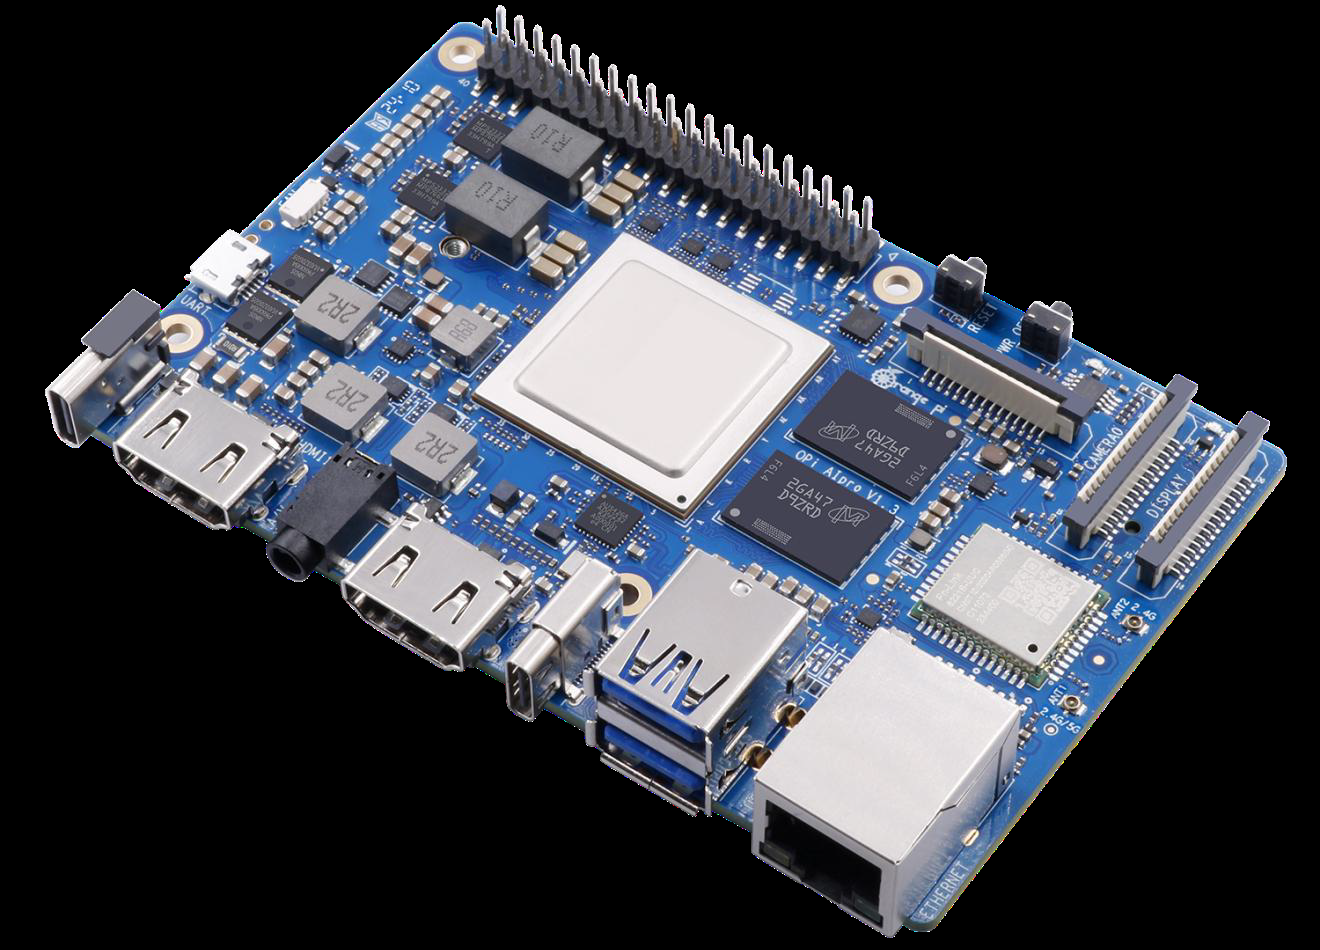
\includegraphics[keepaspectratio,alt={产品图}]{cases/img0/aipro.png}}

\subsection{开发板详细视图}\label{ux5f00ux53d1ux677fux8be6ux7ec6ux89c6ux56fe}

\pandocbounded{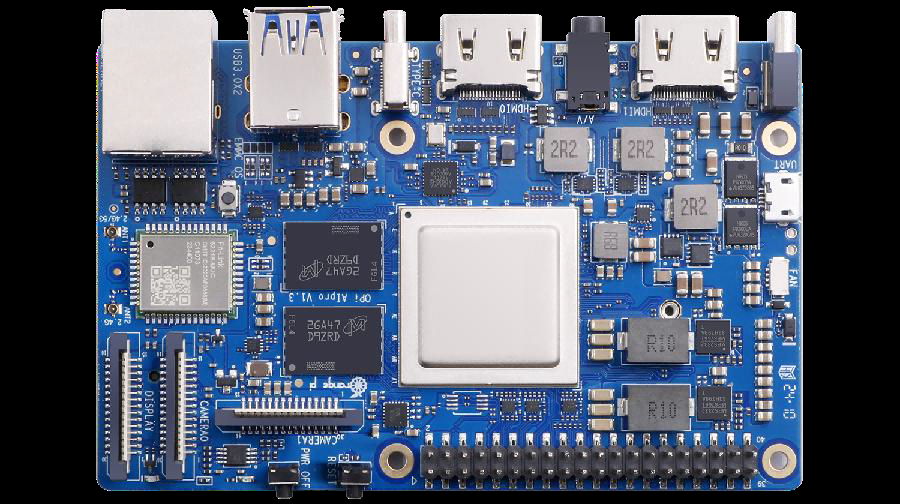
\includegraphics[keepaspectratio,alt={正面视图}]{cases/img0/4.png}}
\pandocbounded{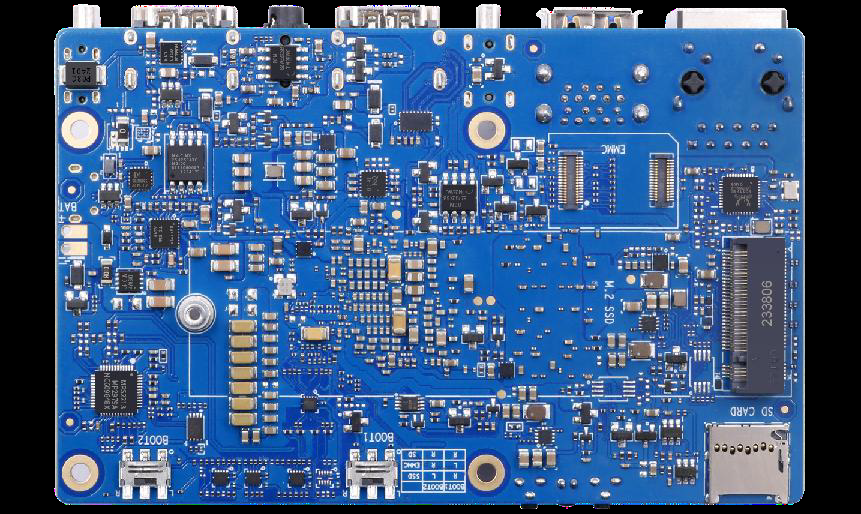
\includegraphics[keepaspectratio,alt={背面试图}]{cases/img0/5.png}}
\pandocbounded{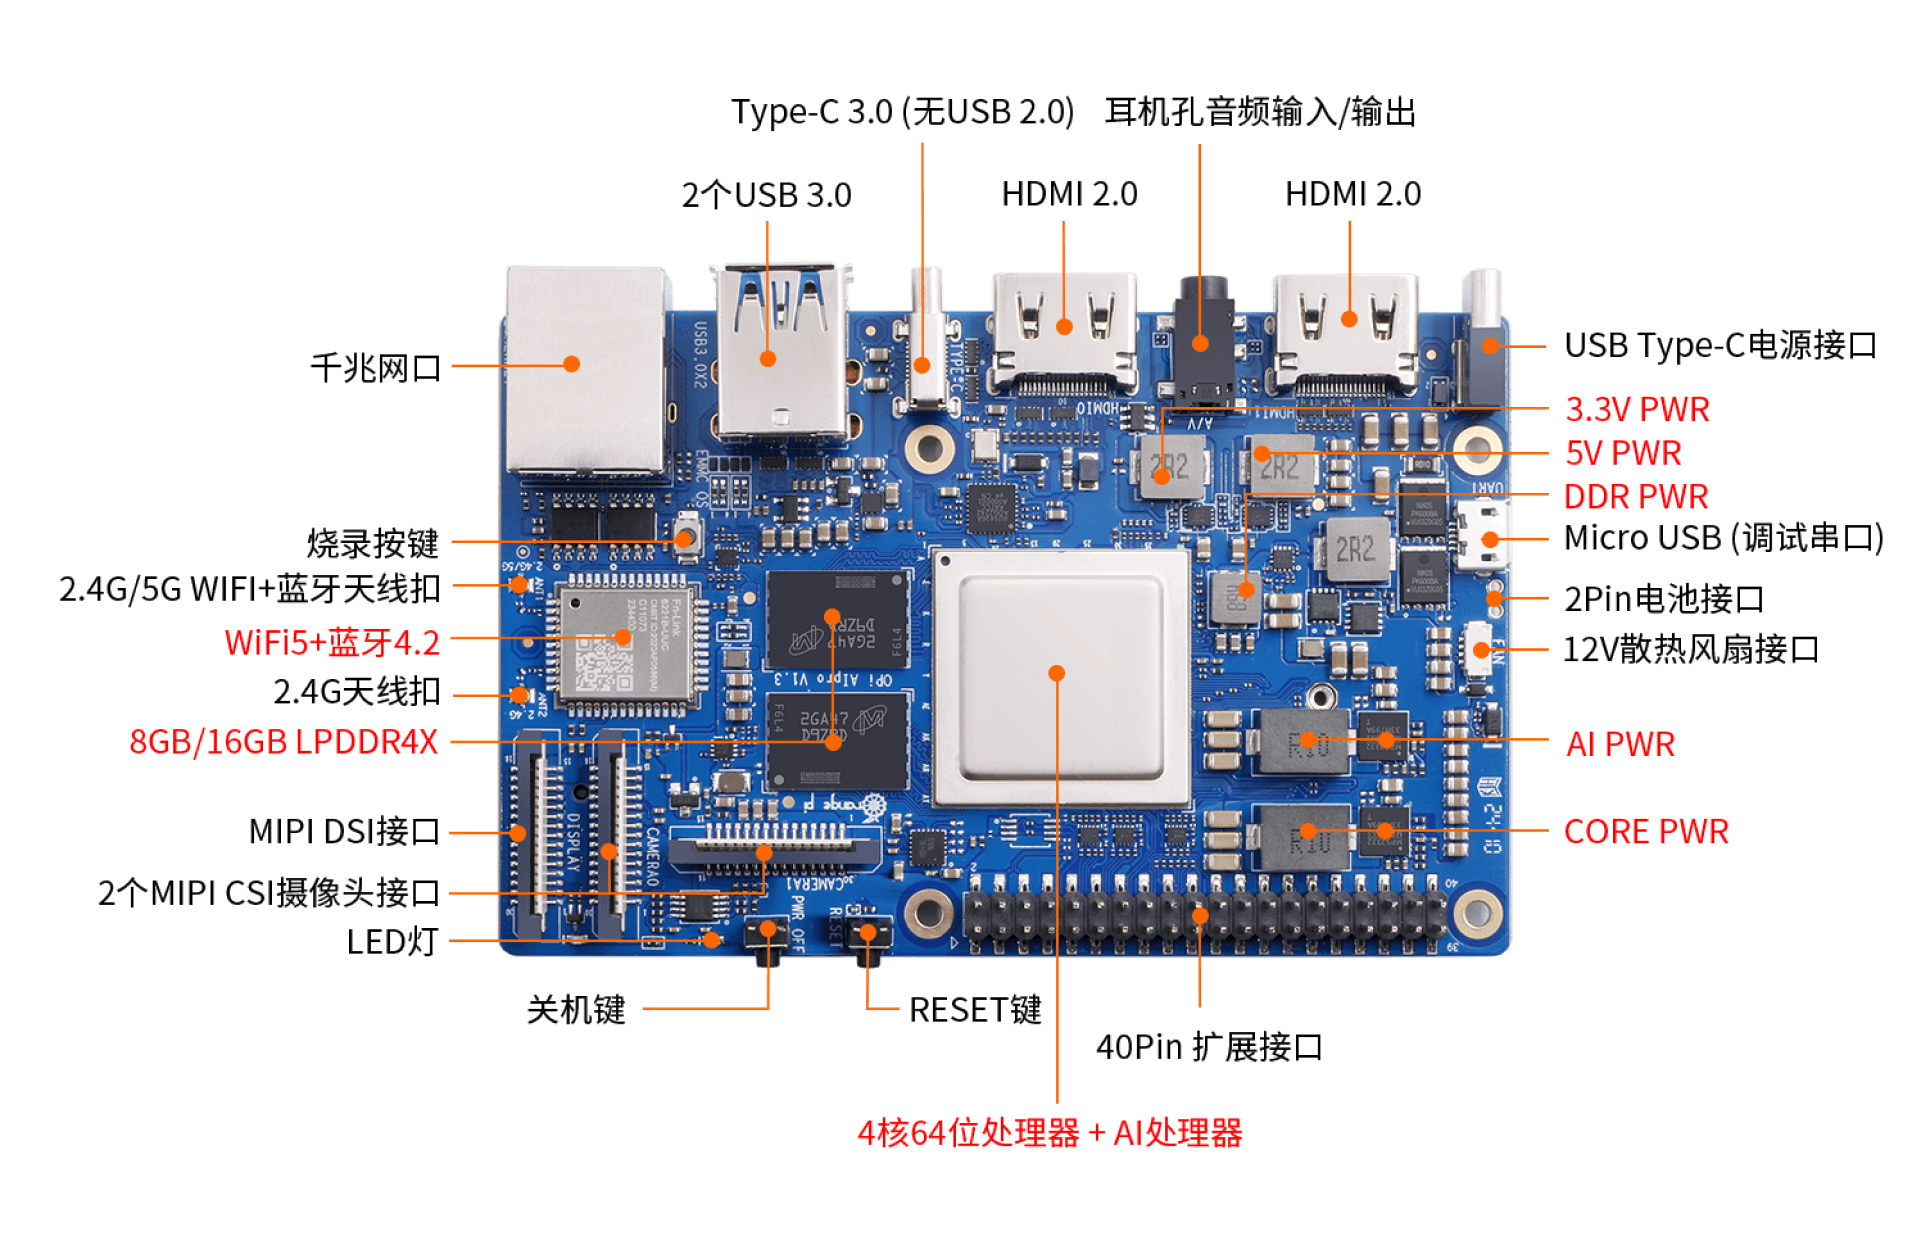
\includegraphics[keepaspectratio,alt={正面标注视图}]{cases/img0/1.png}}
\pandocbounded{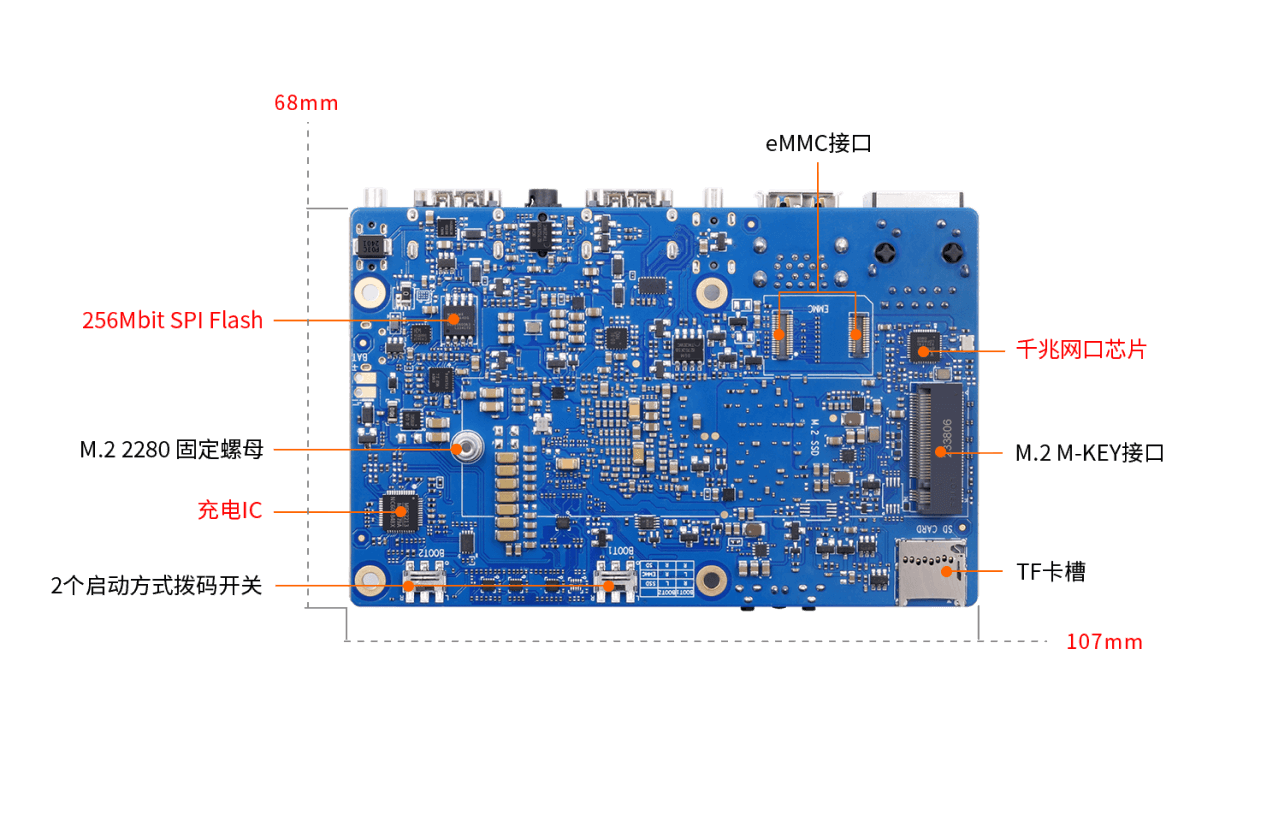
\includegraphics[keepaspectratio,alt={背面标注视图}]{cases/img0/2.png}}
\pandocbounded{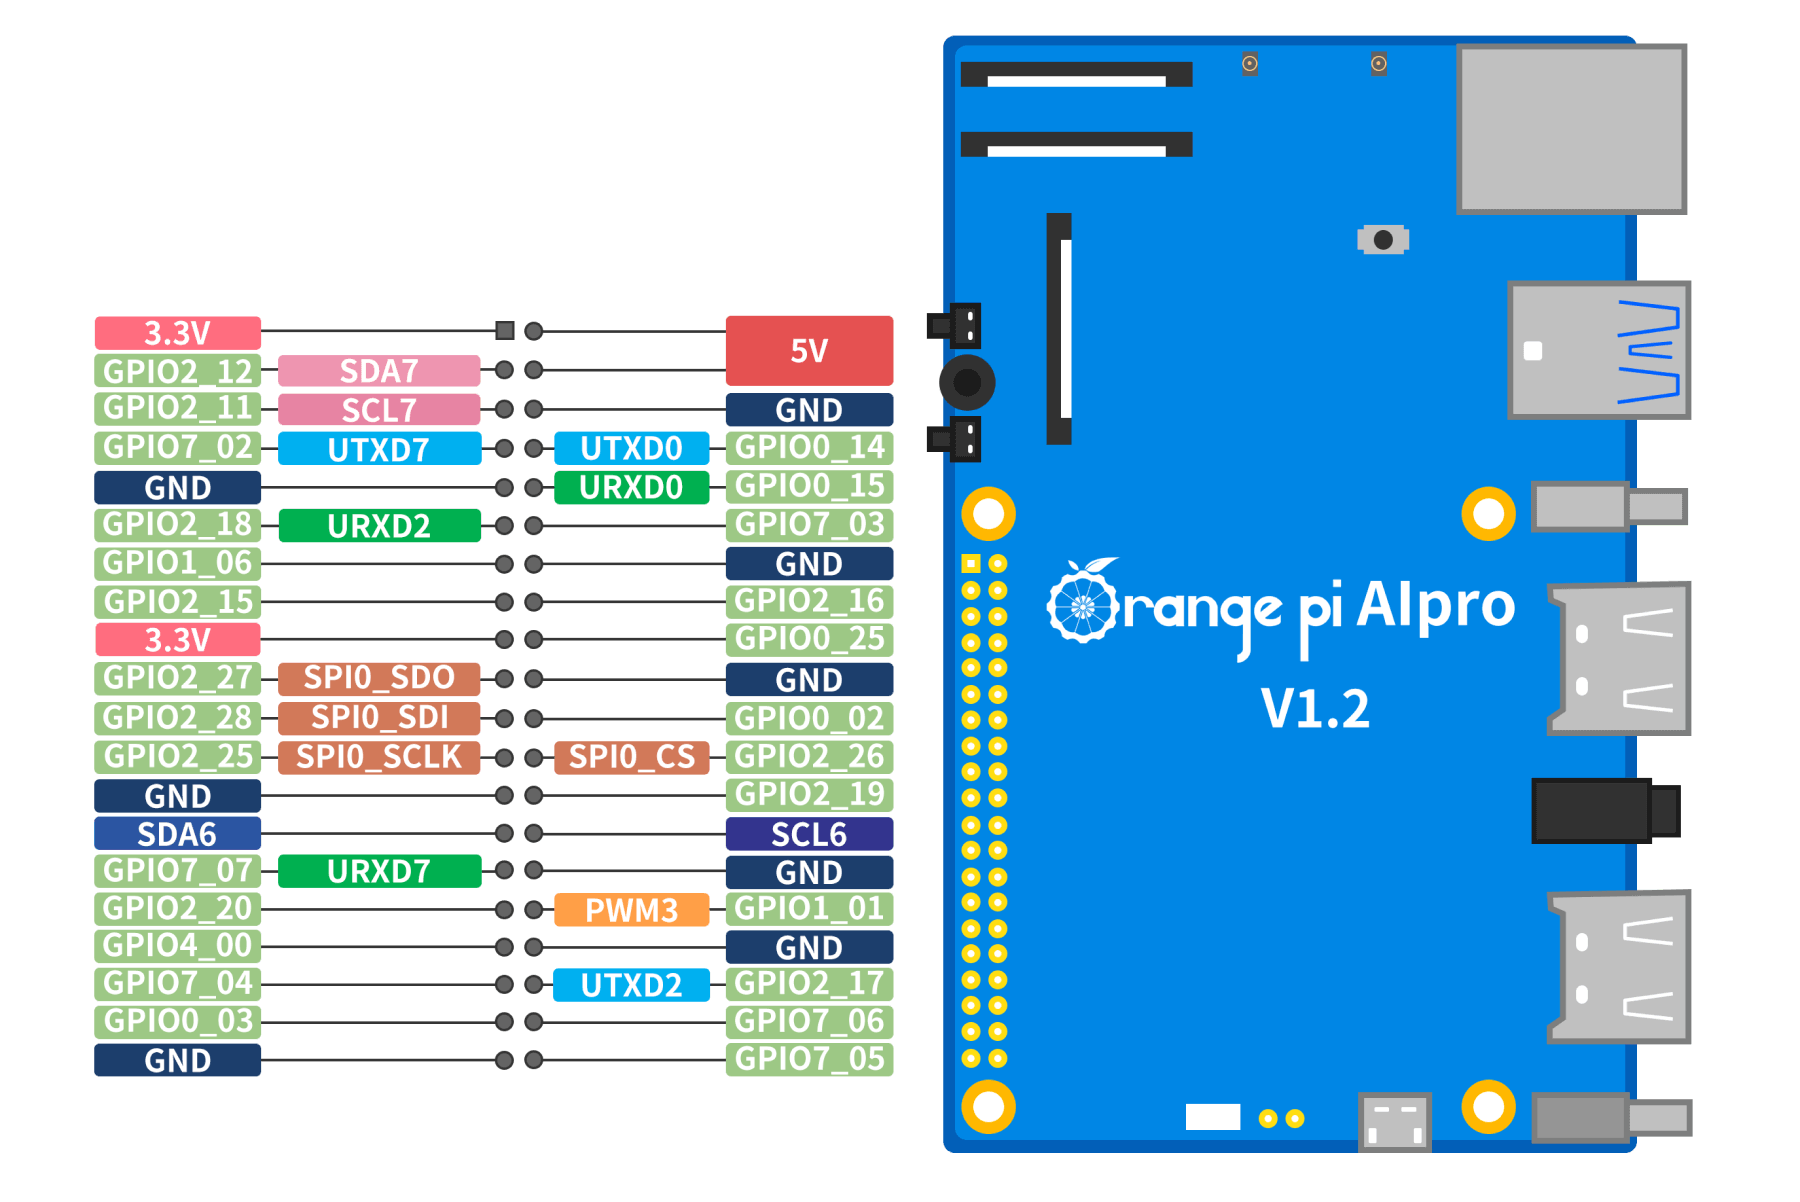
\includegraphics[keepaspectratio,alt={GPIO接口定义}]{cases/img0/3.png}}

\subsection{开发板硬件规格}\label{ux5f00ux53d1ux677fux786cux4ef6ux89c4ux683c}

\begin{center}\rule{0.5\linewidth}{0.5pt}\end{center}

\subsection{所需配件}\label{ux6240ux9700ux914dux4ef6}

\begin{enumerate}
\def\labelenumi{\arabic{enumi}.}
\item
  TF卡
  容量最小为32GB,速率为Class10级以上的闪迪品牌的TF卡,如下图所示。建议使用64G及以上的TF卡,以避免在开发过程中出现磁盘空间不足的问题。
  \pandocbounded{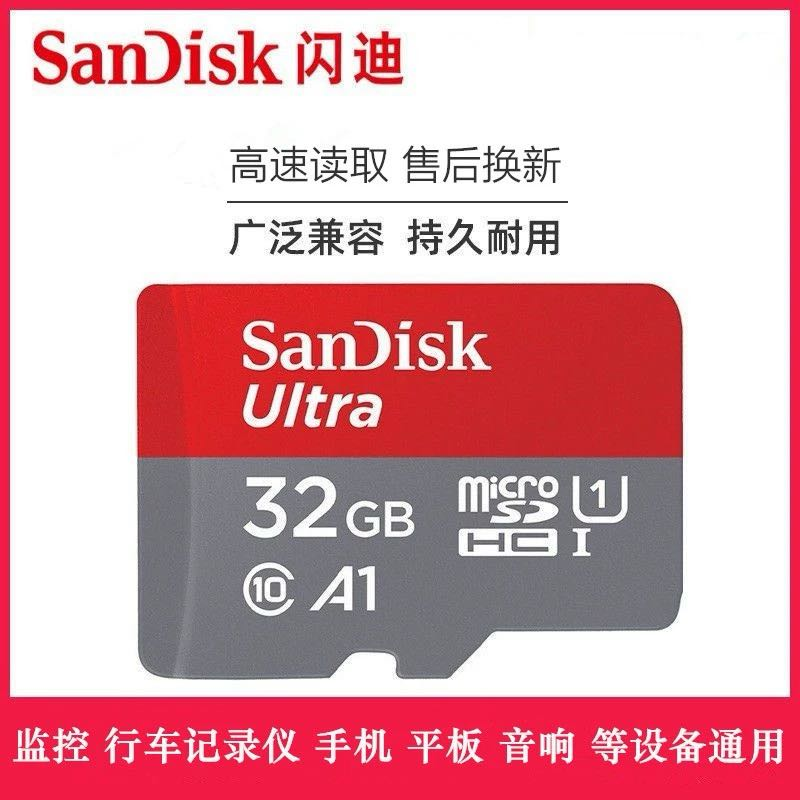
\includegraphics[keepaspectratio,alt={tf卡}]{cases/img0/tf.jpg}}
\item
  TF卡读卡器
  用于读写TF卡,刷写系统,建议选择速率为USB3.0以上的,减少系统刷写的等待时间。
  \pandocbounded{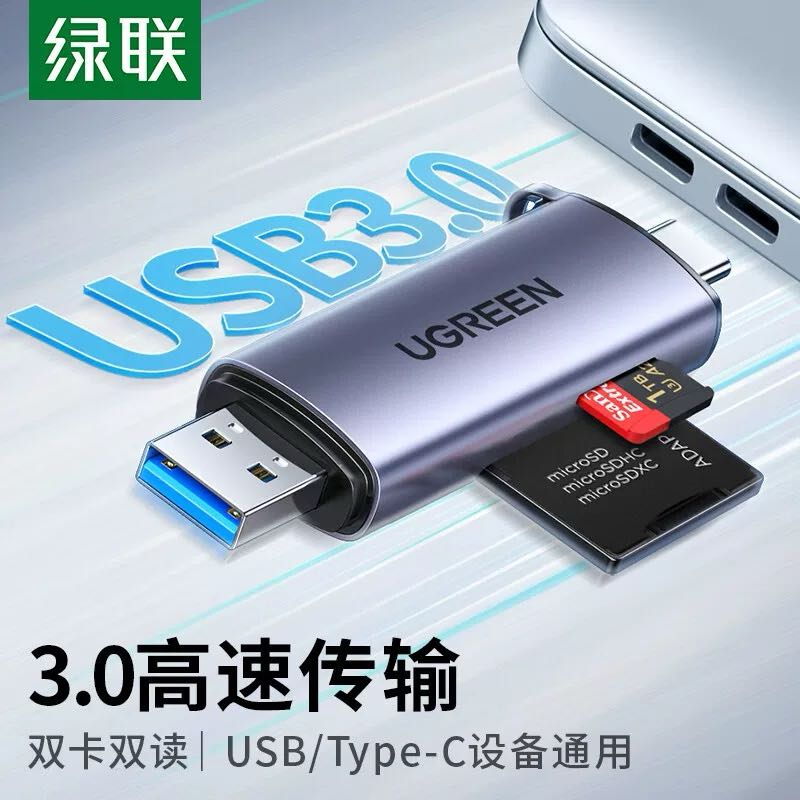
\includegraphics[keepaspectratio,alt={读卡器}]{cases/img0/reader.jpg}}
\item
  HDMI线或HDMI转mini-HDMI线
  主要取决于显示器的接口类型该开发板的视频输出接口为标准HDMI接口。
  \pandocbounded{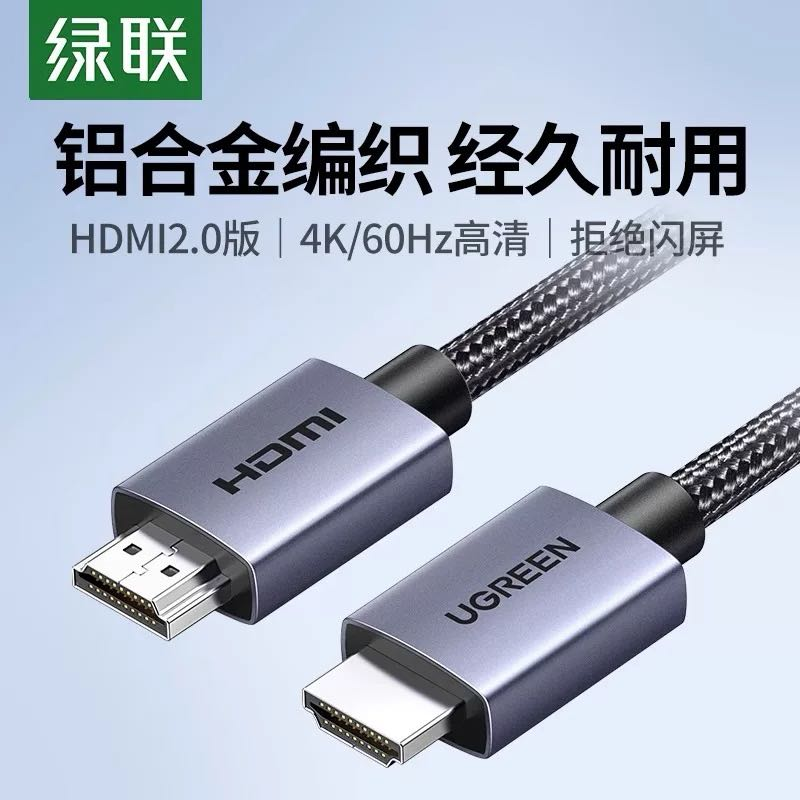
\includegraphics[keepaspectratio,alt={HDMI}]{cases/img0/hdmi.jpg}}
  \pandocbounded{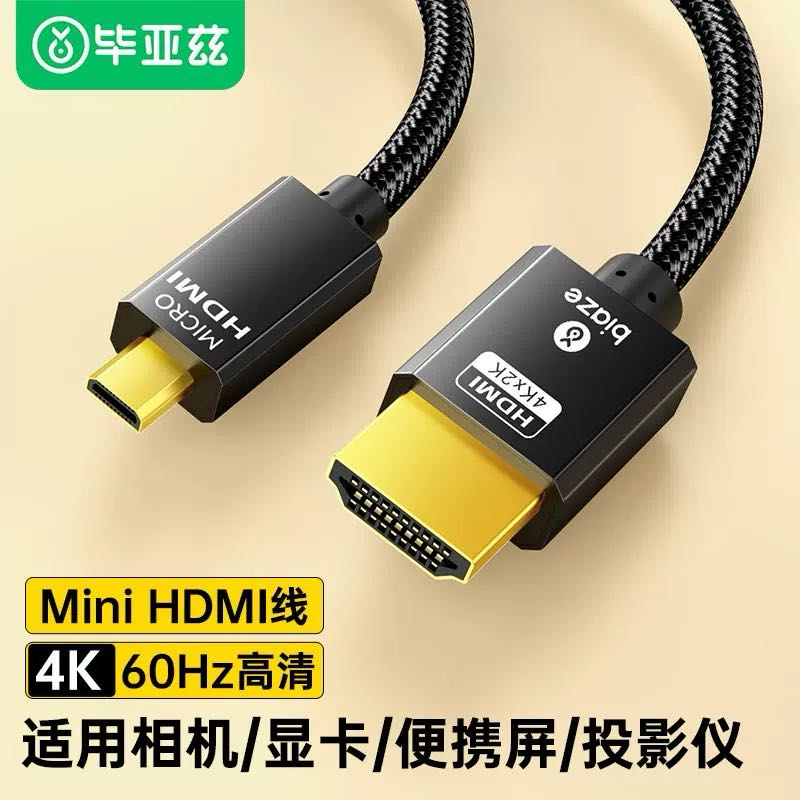
\includegraphics[keepaspectratio,alt={Mini HDMI}]{cases/img0/minihdmi.jpg}}
\item
  电源 该开发板的电源输入为PD
  20V,需要搭配支持PD协议20V挡位的65W电源适配器。
  \pandocbounded{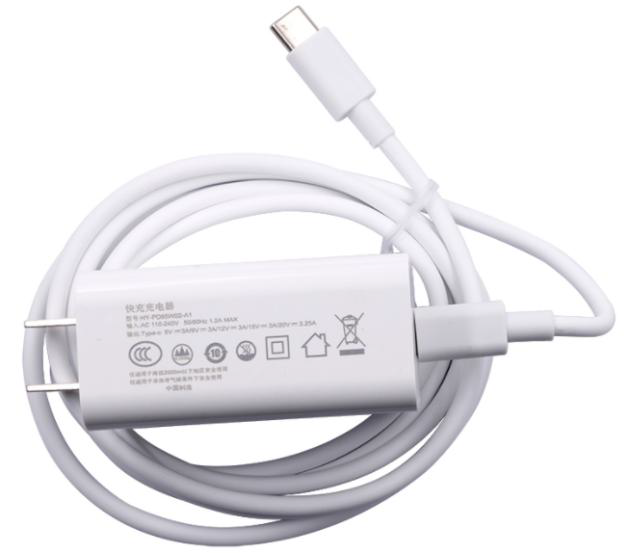
\includegraphics[keepaspectratio,alt={PD电源}]{cases/img0/power.png}}
\item
  USB接口的鼠标以及键盘 在无远程访问的条件下对开发板进行本地调试。
  \pandocbounded{
\includegraphics[keepaspectratio,alt={鼠标}]{cases/img0/mouse.png}}
\item
  金属配套外壳 用于保护开发板硬件。
  \pandocbounded{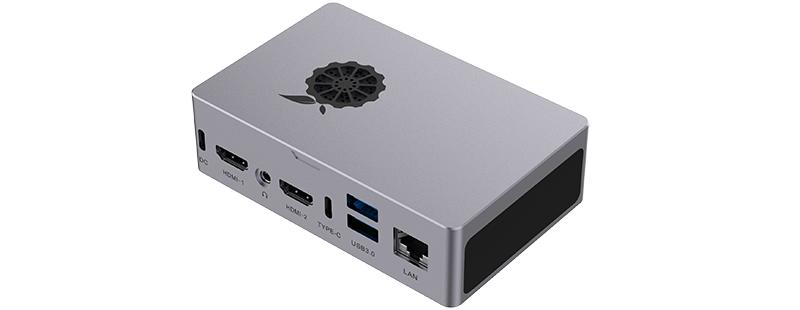
\includegraphics[keepaspectratio,alt={外壳}]{cases/img0/cover.png}}
\item
  12V散热风扇以及散热鳍块
  开发板的风扇接口为2pin,输出电压为12v,支持PWM调速。由于该开发板的CPU发热较大,强烈建议安装主动扇热设备。
  \pandocbounded{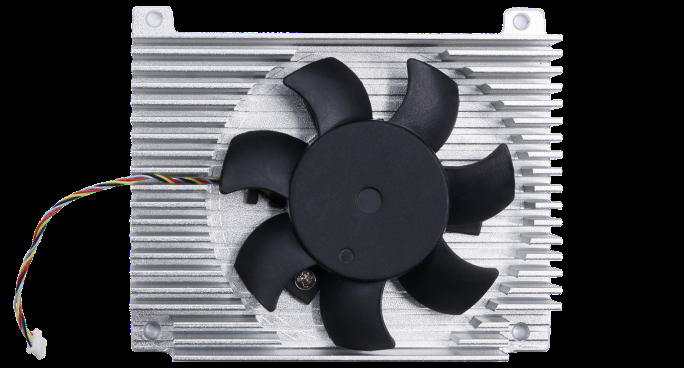
\includegraphics[keepaspectratio,alt={风扇}]{cases/img0/fan.png}}
\item
  Type-C转USB 3.0转接线(可选) OrangePi
  AIPro开发板具有一个Type-C接口,协议为USB3.0(不支持USB
  2.0),可外接支持USB3.0以上协议的外置设备。
  \pandocbounded{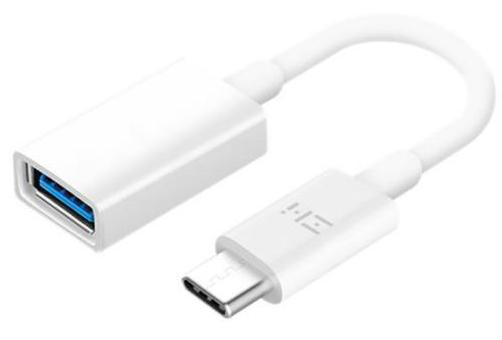
\includegraphics[keepaspectratio,alt={转接线}]{cases/img0/otg.png}}
\item
  M.2接口 2280规格的PCIe Nvme SSD(可选)
  开发板的背部设计有M.2接口,可外接一个M.2的SSD作为开发板的系统盘或者存储。
  \pandocbounded{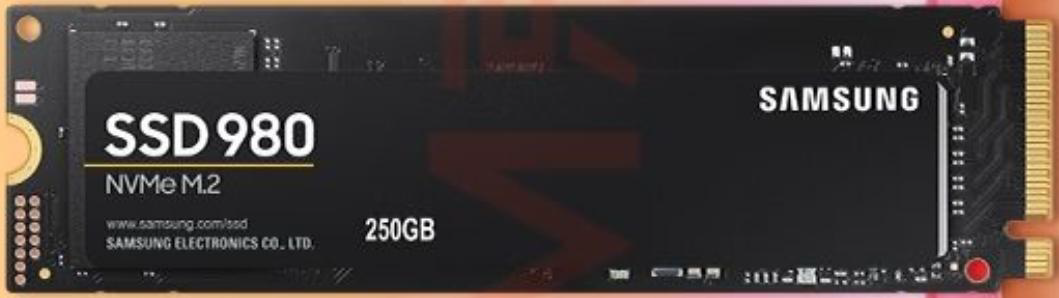
\includegraphics[keepaspectratio,alt={nvme ssd}]{cases/img0/nvme.png}}
\item
  M.2接口 2280规格的Sata Ngff SSD(可选)
  同样,开发板的M.2接口不仅支持PCIe协议,也支持Sata协议,因此也可以使用Sata协议的SSD。
  \pandocbounded{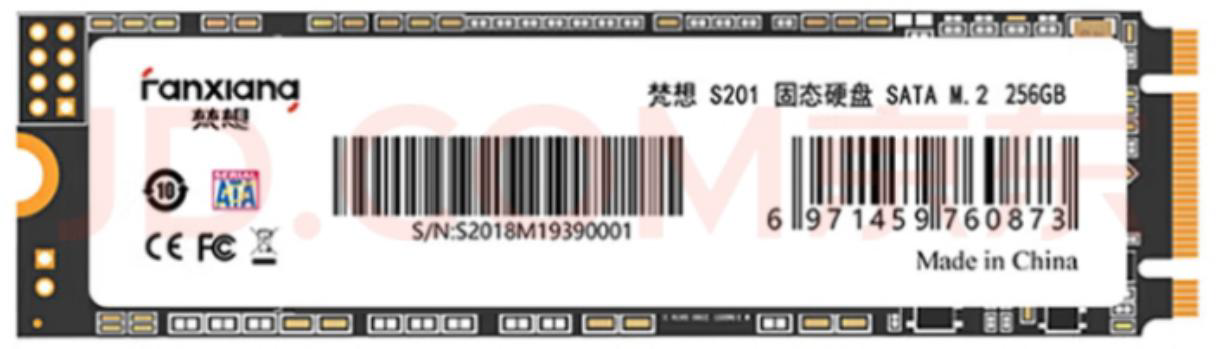
\includegraphics[keepaspectratio,alt={ngff ssd}]{cases/img0/ngff.png}}
\item
  香橙派的eMMC模块(可选)
  eMMC(嵌入式多媒体卡)是一种集成了闪存和控制器的低成本存储解决方案,主要用于智能手机、平板电脑和低端笔记本电脑等消费电子产品。其读写速度适中(100-400MB/s),比传统机械硬盘快但不及固态硬盘(SSD),具有体积小、功耗低和易于集成的特点。开发板支持使用eMMC模块作为存储,但需要额外购置eMMC模块。
  \pandocbounded{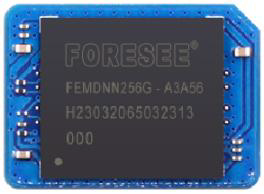
\includegraphics[keepaspectratio,alt={emmc正面}]{cases/img0/emmc1.png}}
  \pandocbounded{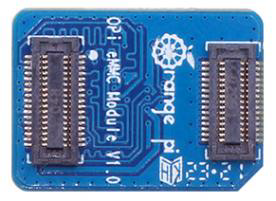
\includegraphics[keepaspectratio,alt={emmc背面}]{cases/img0/emmc2.png}}
\item
  USB摄像头模块(可选) 可用于图像识别、视频通话等多方面用途。
  \pandocbounded{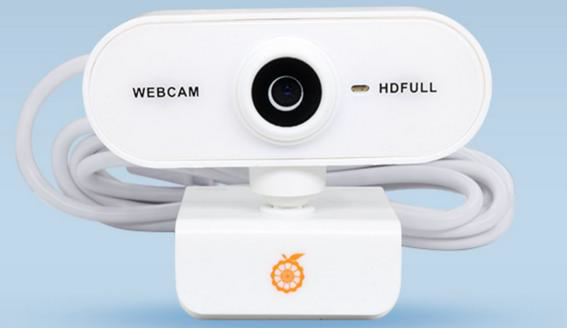
\includegraphics[keepaspectratio,alt={摄像头}]{cases/img0/camera.png}}
\item
  网线(可选)
  开发板自带有wifi模块可用于连接wifi,若需要更稳定的网络连接,建议使用网线连接。
  \pandocbounded{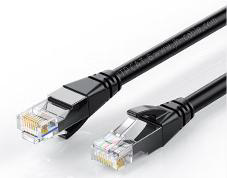
\includegraphics[keepaspectratio,alt={网线}]{cases/img0/cable.png}}
\item
  树莓派IMX219型号摄像头(MIPI-CSI)(可选)
  开发板带有两个MIPI-CSI接口,可以兼容树莓派的MIPI摄像头,无需占用USB接口。
  \pandocbounded{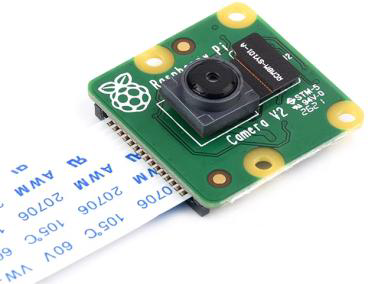
\includegraphics[keepaspectratio,alt={MIPI-CSI摄像头}]{cases/img0/csi.png}}
\item
  树莓派5寸MIPI LCD显示屏(可选)
  开发板带有一个MIPI-DSI显示输出接口,可以直接驱动MIPI的显示屏,而无需外接显示器。
  \pandocbounded{
\includegraphics[keepaspectratio,alt={MIPI显示器}]{cases/img0/dsi.png}}
\item
  Micro USB数据线(可选) 开发板自带了CH343P芯片,将UART转发为Micro
  USB接口,若需要使用串口对开发板进行调试,则需要使用Micro USB数据线。
  \pandocbounded{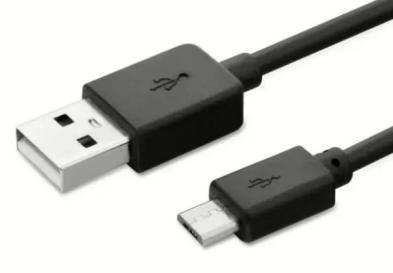
\includegraphics[keepaspectratio,alt={Micro USB数据线}]{cases/img0/microusb.png}}
\end{enumerate}

\subsection{下载开发板的系统镜像}\label{ux4e0bux8f7dux5f00ux53d1ux677fux7684ux7cfbux7edfux955cux50cf}

作为华为生态中重要的一员,开发板不仅支持Ubuntu系统,也支持openEuler系统,但由于开发板自身并无存储,我们在使用开发板的过程中需要使用电脑对TF卡进行系统的刷写,建议使用安装有Windows11
或 Ubuntu22.04以上版本的PC。

首先,打开香橙派官网的\href{http://www.orangepi.cn/html/hardWare/computerAndMicrocontrollers/service-and-support/Orange-Pi-AIpro.html}{技术支持界面}。\pandocbounded{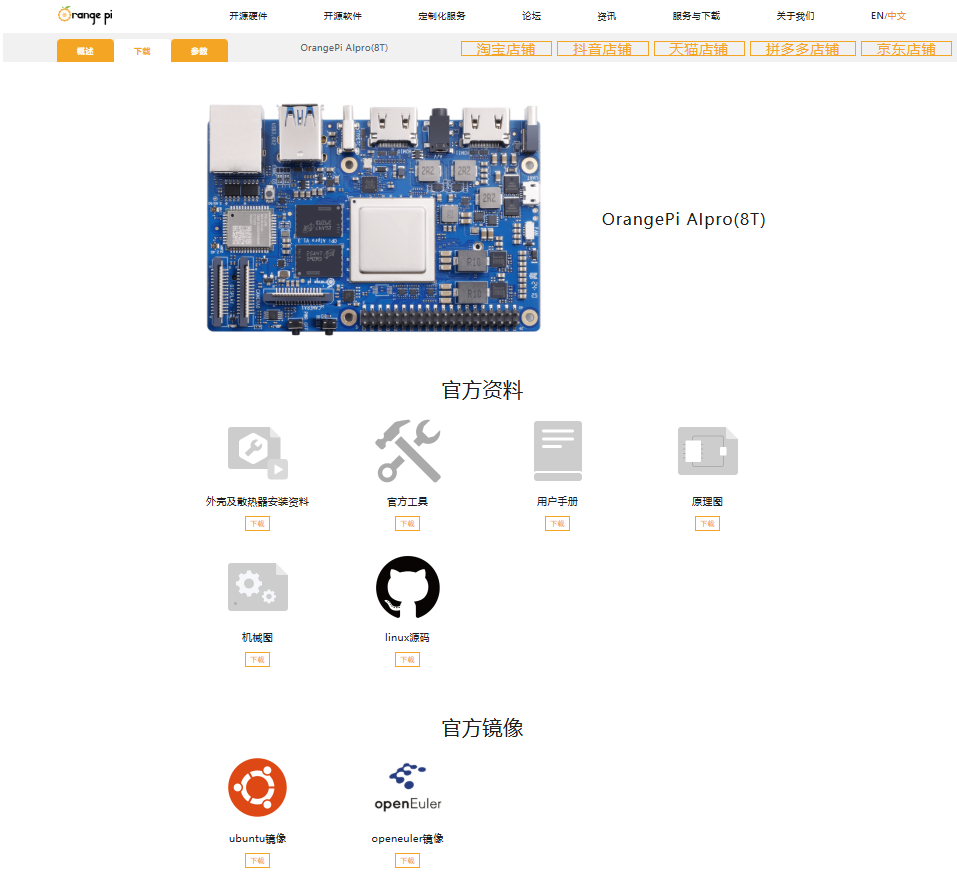
\includegraphics[keepaspectratio,alt={技术支持页面}]{cases/img0/技术支持.png}}

向下滑动网页,找到官方镜像部分,分为Ubuntu和openEuler两个部分,两个系统都是官方为我们编译完成的,且预装了部分昇腾NPU的应用环境以及软件,非常方便新手用户上手使用。
\pandocbounded{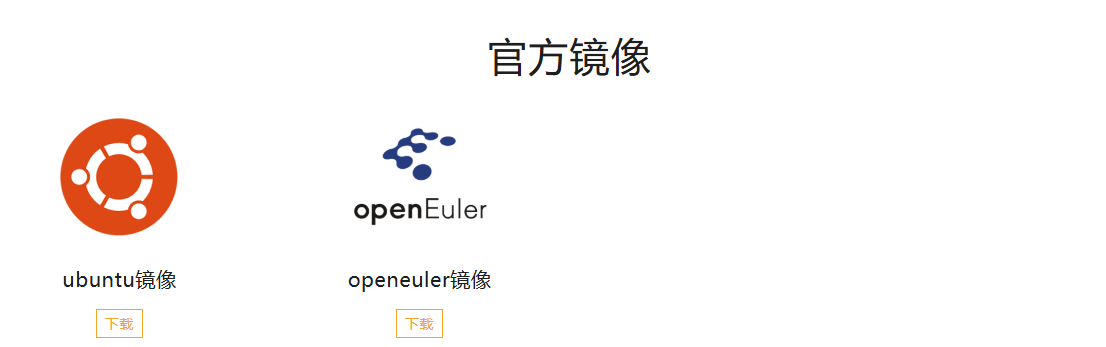
\includegraphics[keepaspectratio,alt={官方镜像}]{cases/img0/官方镜像.png}}

\subsubsection{Ubuntu}\label{ubuntu}

\begin{enumerate}
\def\labelenumi{\arabic{enumi}.}
\tightlist
\item
  点击下载\pandocbounded{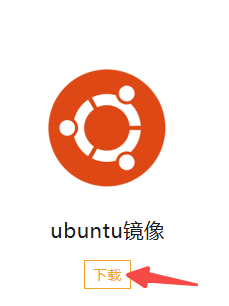
\includegraphics[keepaspectratio,alt={下载}]{cases/img0/download_ubuntu.png}}
\item
  复制提取码并跳转\pandocbounded{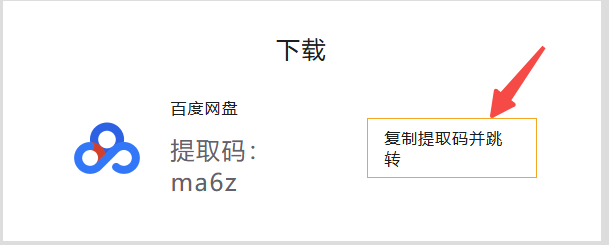
\includegraphics[keepaspectratio,alt={跳转}]{cases/img0/copyandjump.png}}
\item
  打开百度网盘的链接后有一个命名为Ubuntu的文件夹,点开该文件夹\pandocbounded{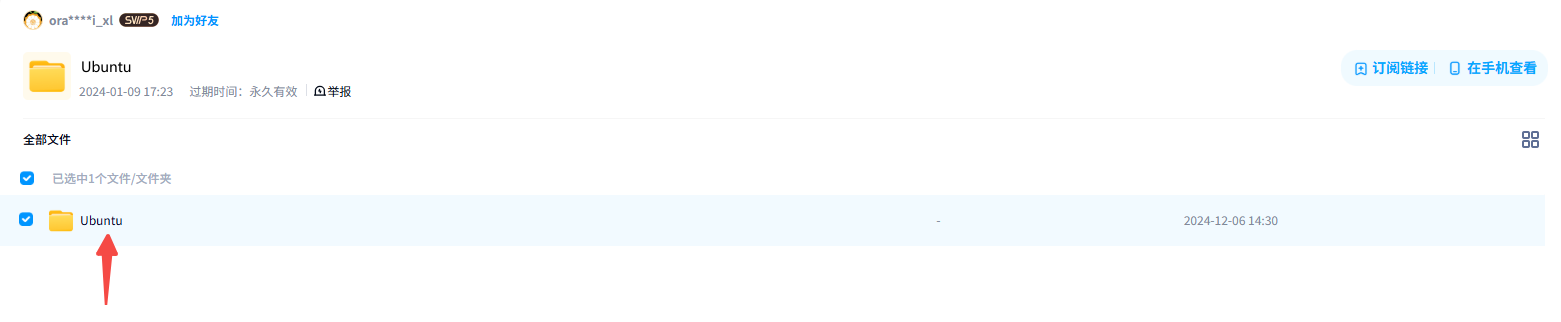
\includegraphics[keepaspectratio,alt={文件夹}]{cases/img0/folder.png}}
\item
  文件夹中,后缀为.xz的文件是镜像压缩包文件,.sha文件是压缩包的md5校验码文件,用于校验镜像包文件是否完整。
\item
  文件夹中的镜像有两种,一种文件名带有Desktop的,是带有GUI图形化界面的,另一种文件名带有minimal的,是不具有图形化界面的,只有命令行界面。建议新学习的用户使用带有desktop的镜像。
  \pandocbounded{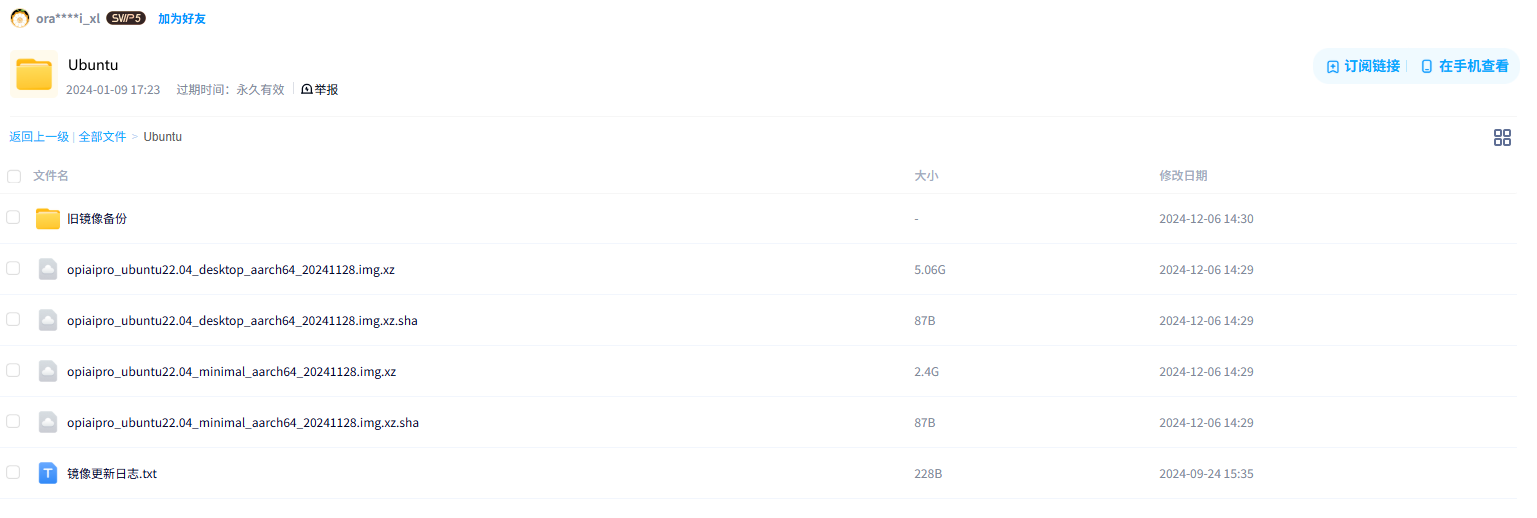
\includegraphics[keepaspectratio,alt={选择镜像}]{cases/img0/chooseubuntu.png}}
\item
  下载后先校验压缩包是否完整,后解压压缩包
\end{enumerate}

\subsubsection{openEuler}\label{openeuler}

\begin{enumerate}
\def\labelenumi{\arabic{enumi}.}
\tightlist
\item
  点击下载\pandocbounded{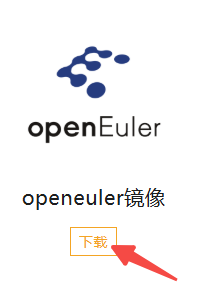
\includegraphics[keepaspectratio,alt={下载}]{cases/img0/download_openeuler.png}}
\item
  复制提取码并跳转\pandocbounded{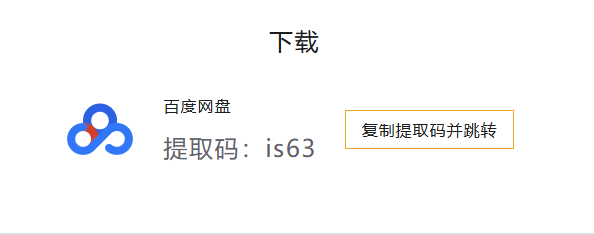
\includegraphics[keepaspectratio,alt={跳转}]{cases/img0/cpjp.png}}
\item
  打开百度网盘的链接后有一个命名为OpenEuler的文件夹,点开该文件夹\pandocbounded{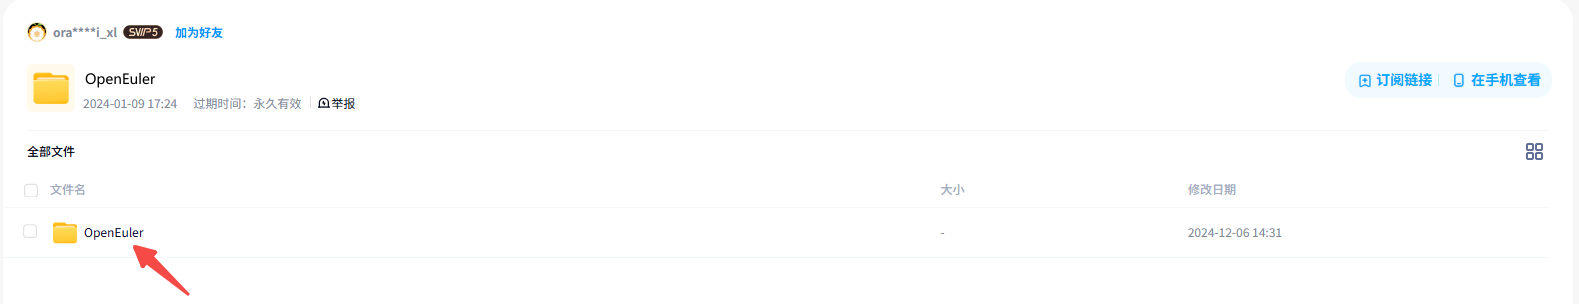
\includegraphics[keepaspectratio,alt={文件夹}]{cases/img0/folderr.png}}
\item
  文件夹中,后缀为.xz的文件是镜像压缩包文件,.sha文件是压缩包的md5校验码文件,用于校验镜像包文件是否完整。
\item
  文件夹中的镜像只有一种,即具有GUI图形化界面的openEuler系统。\pandocbounded{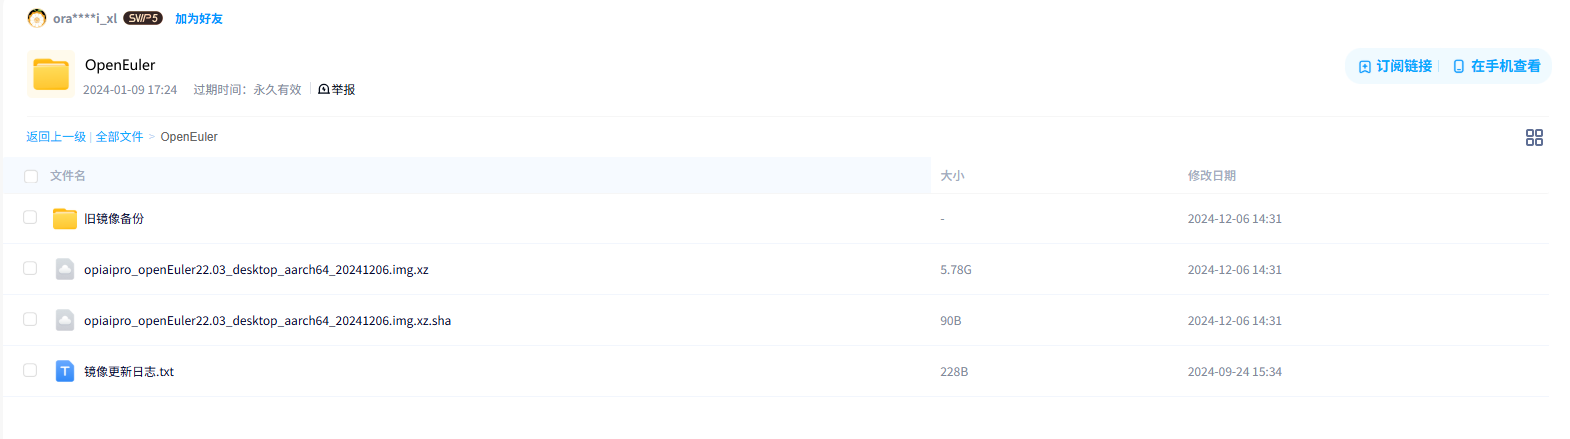
\includegraphics[keepaspectratio,alt={OpenEuler}]{cases/img0/chooseeuler.png}}
\item
  下载后先校验压缩包是否完整,后解压压缩包
\end{enumerate}

\subsubsection{使用md5校验下载的文件}\label{ux4f7fux7528md5ux6821ux9a8cux4e0bux8f7dux7684ux6587ux4ef6}

在Windows系统下,可以使用\passthrough{\lstinline!certutil -hashfile <filename> md5!};在Ubuntu系统下,可以使用\passthrough{\lstinline!md5sum <filename>!};在MacOS系统下,可以使用\passthrough{\lstinline!md5 <filename>!}进行计算,此处以Windows系统为例:在文件夹按住Shift键并单击鼠标右键,选择``在终端(Powershell/命令提示符)中打开''\pandocbounded{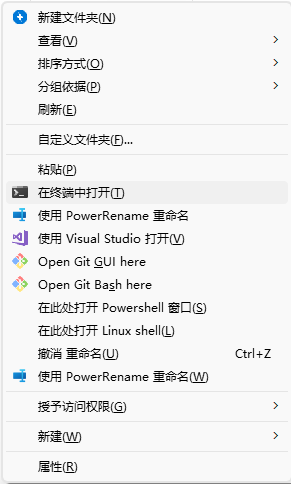
\includegraphics[keepaspectratio,alt={终端}]{cases/img0/shell.png}},然后在打开的窗口中输入\passthrough{\lstinline!certutil -hashfile opiaipro\_ubuntu22.04\_desktop\_aarch64\_20241128.img.xz md5!}\pandocbounded{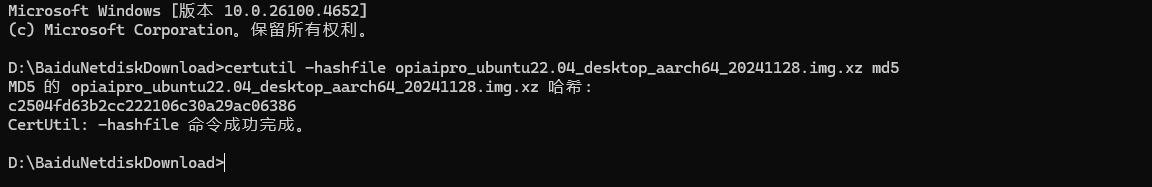
\includegraphics[keepaspectratio,alt={md5校验}]{cases/img0/md5.png}},将得到的md5值与\passthrough{\lstinline!opiaipro\_ubuntu22.04\_desktop\_aarch64\_20241128.img.xz.sha!}文件进行对比,若一致可进行下一步操作,否则需要重新下载。

\subsection{刷写系统到TF卡}\label{ux5237ux5199ux7cfbux7edfux5230tfux5361}

\subsubsection{下载并安装必要的工具}\label{ux4e0bux8f7dux5e76ux5b89ux88c5ux5fc5ux8981ux7684ux5de5ux5177}

\begin{quote}
下载链接:\href{http://www.orangepi.cn/html/hardWare/computerAndMicrocontrollers/service-and-support/Orange-Pi-AIpro.html}{官网}
\href{https://pan.baidu.com/s/1Jho73pw91r5GJD2KijY45Q?pwd=3xuz\#list/path=\%2F}{百度网盘}
1. SD Card Formatter
这个是TF卡的快速格式化工具,在每次需要刷写系统之前,都必须先对TF卡进行格式化操作,若不格式化在后续的刷写系统过程中有较大概率出错。
2. balenaEther 这个是系统镜像的刷写工具,用于刷写img镜像文件进入TF卡。
\end{quote}

\subsubsection{格式化TF卡}\label{ux683cux5f0fux5316tfux5361}

\begin{enumerate}
\def\labelenumi{\arabic{enumi}.}
\tightlist
\item
  将TF卡插入读卡器中,并将读卡器插入电脑
\item
  打开SD Card
  Formatter软件\pandocbounded{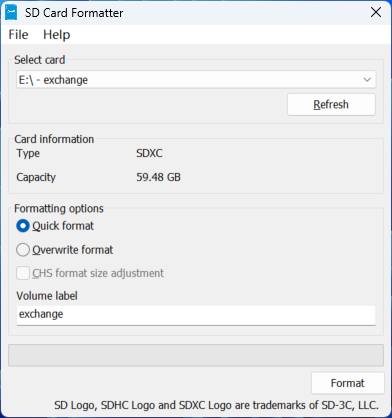
\includegraphics[keepaspectratio,alt={TF卡格式化}]{cases/img0/SDFmt.png}}
\item
  点击右下角Format按键,格式化TF卡\pandocbounded{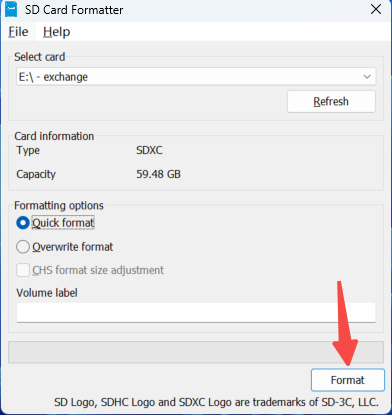
\includegraphics[keepaspectratio,alt={格式化}]{cases/img0/fmt.png}}
  \textgreater{}
  警告内容是关于格式化操作会清除TF卡上原有的所有数据,此处选是\pandocbounded{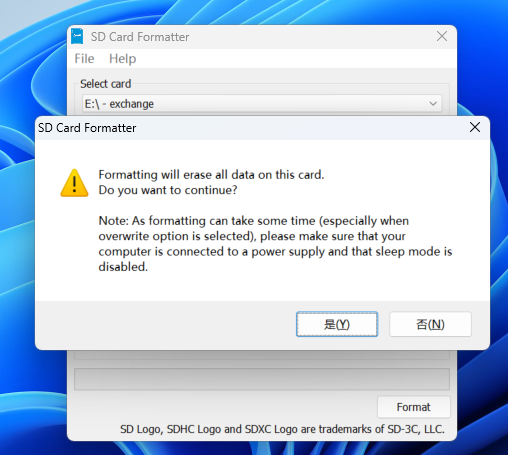
\includegraphics[keepaspectratio,alt={warning}]{cases/img0/warning.png}}
\item
  等待软件格式化完成,并点击确定\pandocbounded{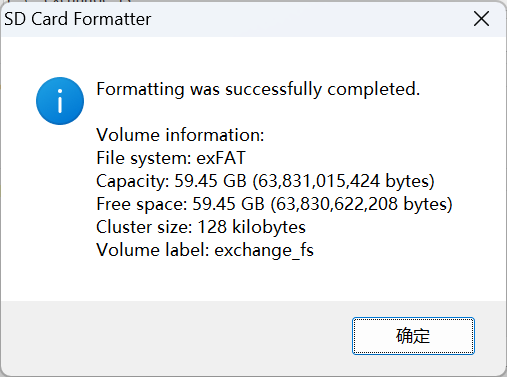
\includegraphics[keepaspectratio,alt={格式化完成}]{cases/img0/fmtfin.png}}
\end{enumerate}

\subsubsection{刷写系统到TF卡(以Ubuntu为例)}\label{ux5237ux5199ux7cfbux7edfux5230tfux5361ux4ee5ubuntuux4e3aux4f8b}

\begin{quote}
此处以刷写Ubuntu为例
\end{quote}

\begin{enumerate}
\def\labelenumi{\arabic{enumi}.}
\tightlist
\item
  打开balenaEther,选择``从文件烧录''\pandocbounded{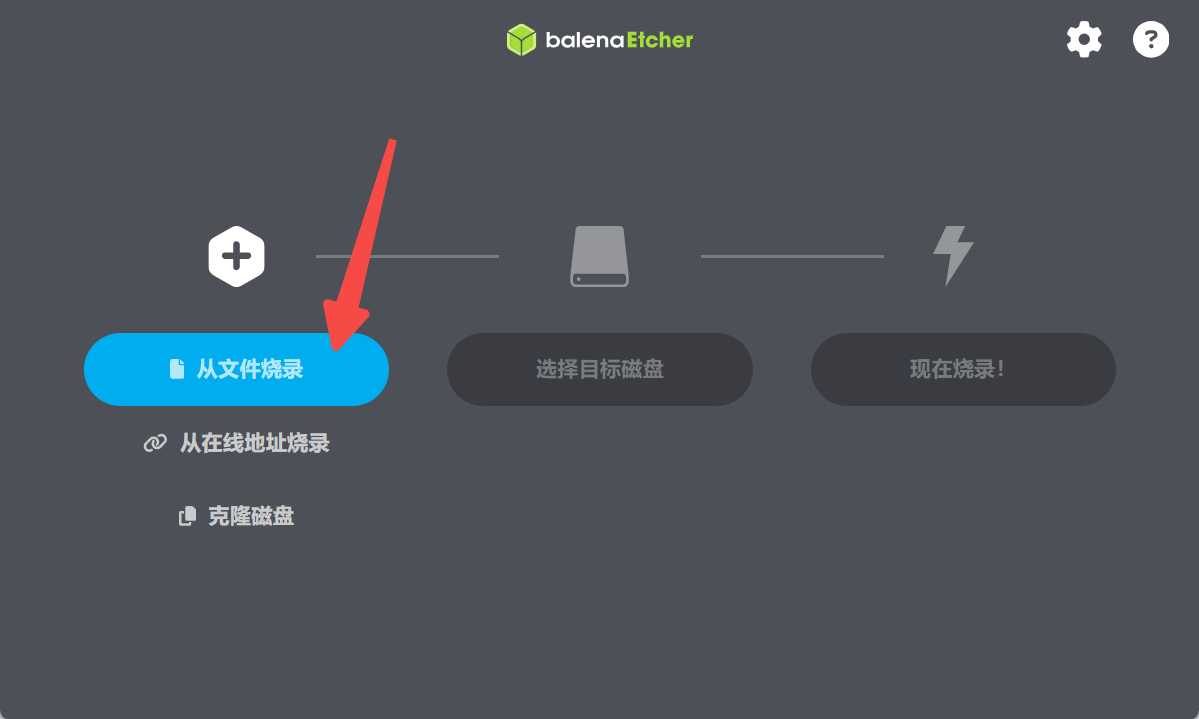
\includegraphics[keepaspectratio,alt={balenaEther}]{cases/img0/ether1.png}}
\item
  选择好要烧录的镜像文件(\textbf{.img}格式),再选择目标磁盘为TF卡对应的位置,如图中名称为``SDXC
  Card''的位置,选中并选择``选定1''。\pandocbounded{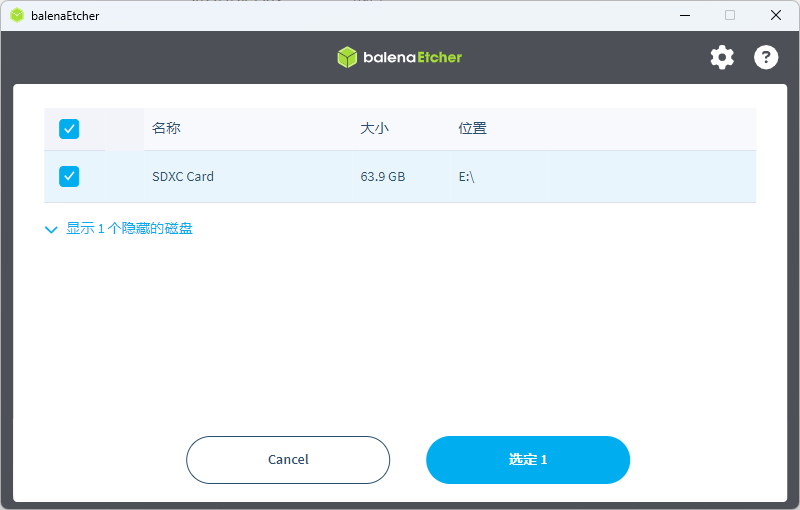
\includegraphics[keepaspectratio,alt={选择磁盘}]{cases/img0/chooseether.png}}
\item
  点击``现在烧录!'',耐心等待烧录完成。\pandocbounded{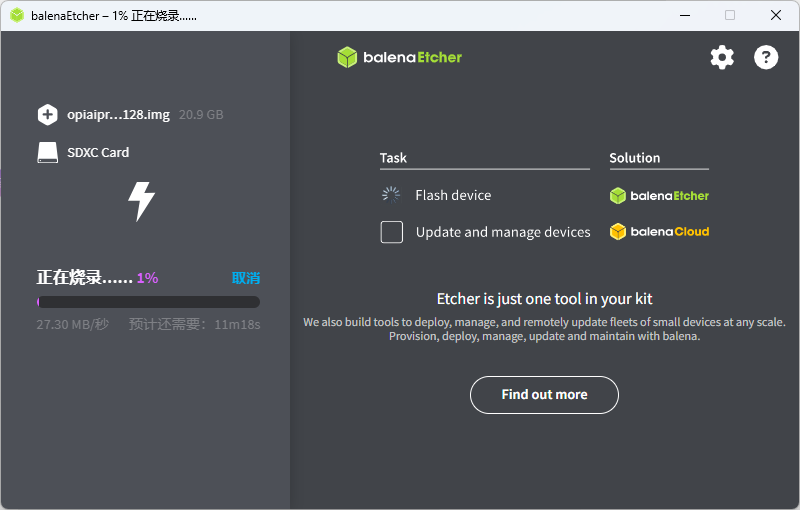
\includegraphics[keepaspectratio,alt={烧录过程}]{cases/img0/dd.png}}
\item
  烧录完成后进入校验过程,也请耐心等待。\pandocbounded{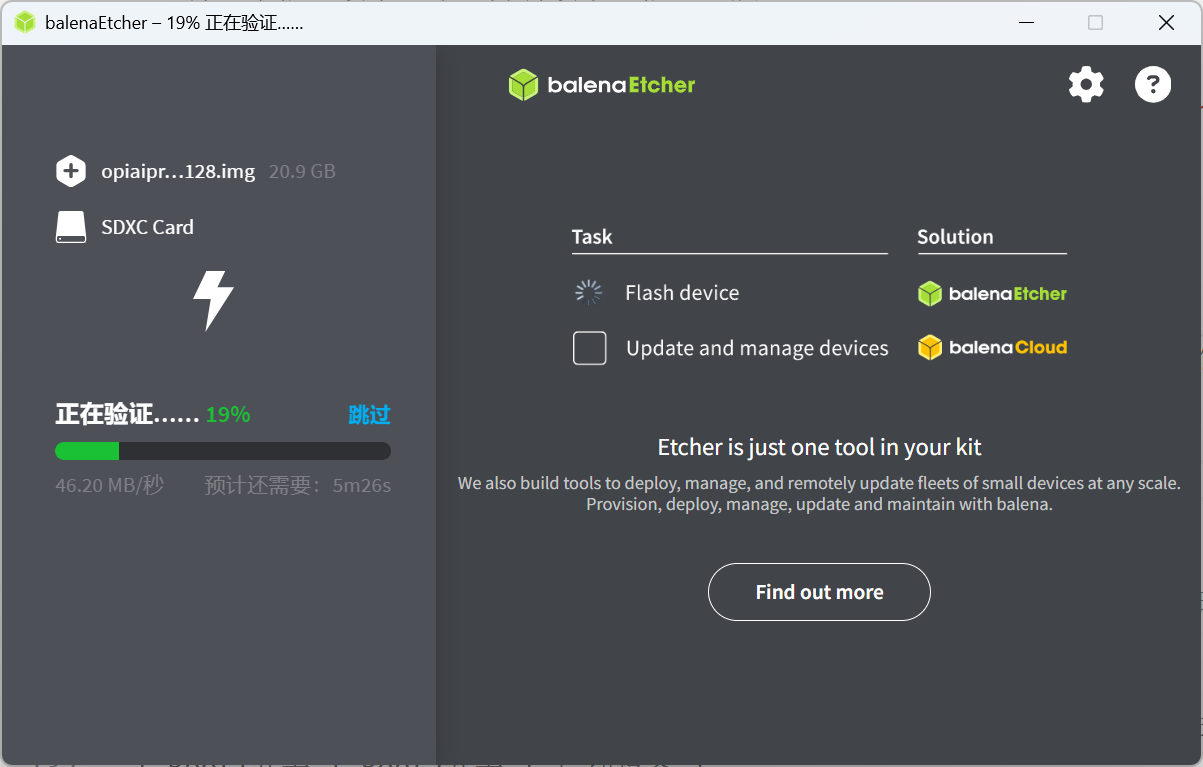
\includegraphics[keepaspectratio,alt={校验过程}]{cases/img0/val.png}}
\item
  烧录完成后即可关闭程序,并安全弹出TF卡\pandocbounded{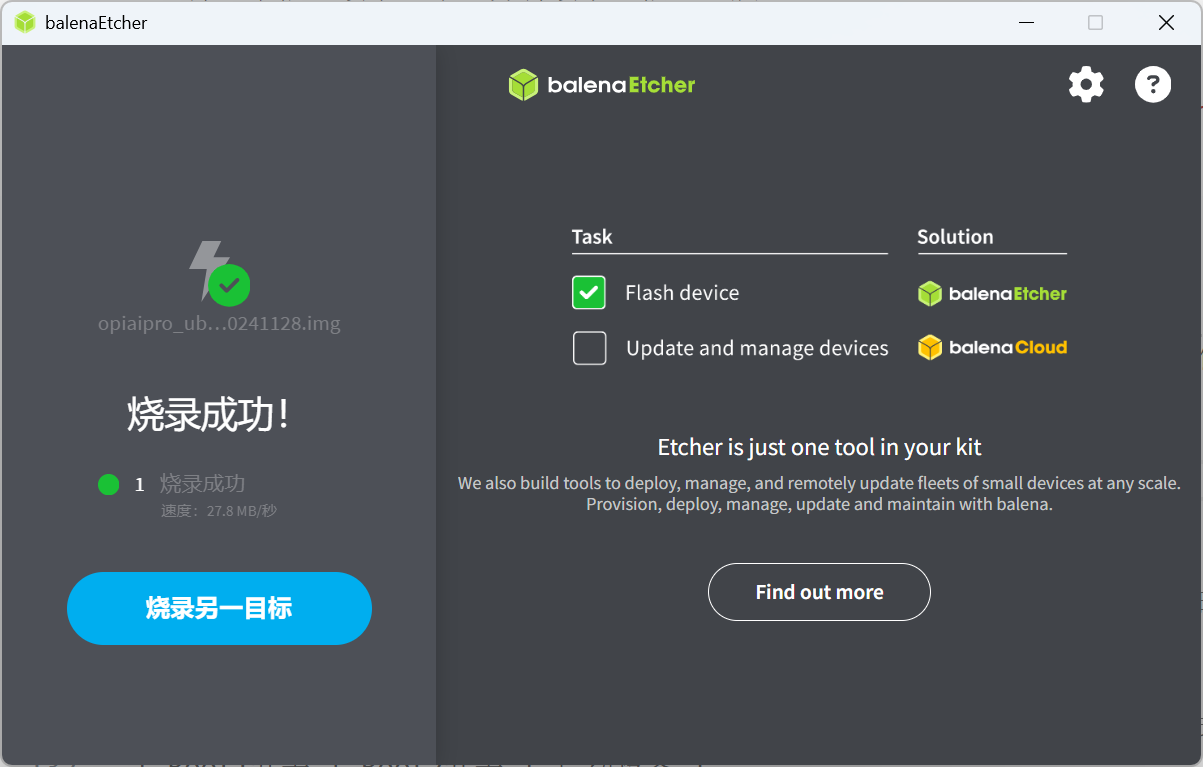
\includegraphics[keepaspectratio,alt={完毕}]{cases/img0/finish.png}}
\end{enumerate}

\subsubsection{刷写系统到eMMC}\label{ux5237ux5199ux7cfbux7edfux5230emmc}

由于板上并不自带有eMMC模块,若要想使用需要额外购买香橙派的eMMC模块,此处暂时不列入参考,若需使用,请查阅香橙派的用户手册。

\subsubsection{刷写系统到SSD}\label{ux5237ux5199ux7cfbux7edfux5230ssd}

开发板带有M.2接口,可以使用SSD作为启动设备。但SSD需要自行准备,且根据香橙派的兼容性说明,该开发版仅支持少数品牌的SSD,因此不推荐使用SSD作为系统安装位置。

\subsubsection{调整设备启动方式的拨码开关}\label{ux8c03ux6574ux8bbeux5907ux542fux52a8ux65b9ux5f0fux7684ux62e8ux7801ux5f00ux5173}

开发板支持多种启动方式,包括TF卡、eMMC以及M.2
SSD,当这些存储设备都同时存在时,需要让开发板选定一个存储设备作为启动来源。

\begin{figure}
\centering
\pandocbounded{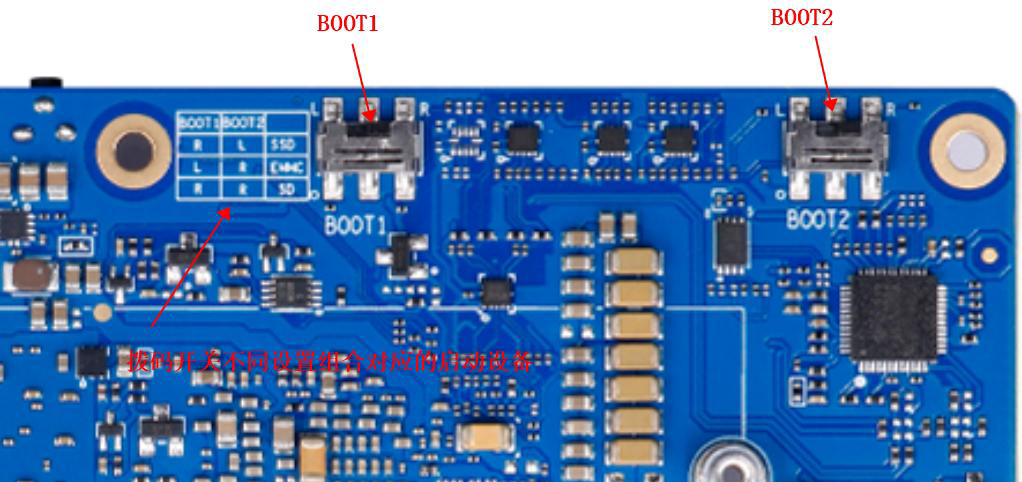
\includegraphics[keepaspectratio,alt={boot开关}]{cases/img0/bootswitch.png}}
\caption{boot开关}
\end{figure}

两个开关都有左、右两种状态,因此共有4种状态,但是目前开发板仅使用3种模式,对应的参数表如下:

\begin{longtable}[]{@{}ccc@{}}
\toprule\noalign{}
Boot1开关 & Boot2开关 & 启动设备 \\
\midrule\noalign{}
\endhead
\bottomrule\noalign{}
\endlastfoot
左 & 左 & 未使用 \\
右 & 右 & TF卡 \\
左 & 右 & eMMC \\
右 & 左 & M.2 SSD (Nvme或Ngff) \\
\end{longtable}

切换拨码开关后,必须要将开发板完全断电再重新上电才能使新的启动配置生效,使用RESET按键重启则不会使新的启动配置生效。

\subsection{启动开发板(Ubuntu)}\label{ux542fux52a8ux5f00ux53d1ux677fubuntu}

\begin{itemize}
\tightlist
\item
  图形化界面
\end{itemize}

\begin{enumerate}
\def\labelenumi{\arabic{enumi}.}
\tightlist
\item
  将系统刷写完成的TF卡从读卡器中取出,插入开发板的TF卡插槽中,并确保两个启动开关的位置均在右边,接入HDMI数据线到靠近USB3.0接口的HDMI0接口,然后将Type-C电源线插入开发板最边缘的TYPE-C供电口,等待风扇的声音变小以及屏幕出现系统登录界面。
  \pandocbounded{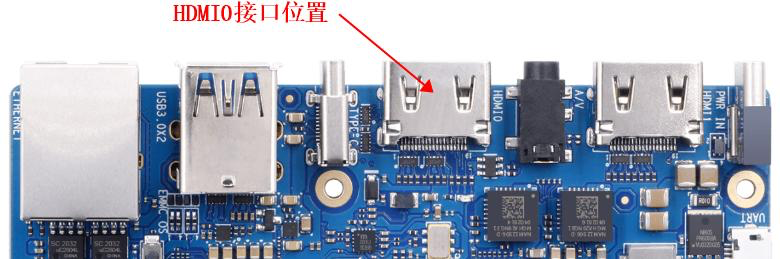
\includegraphics[keepaspectratio,alt={HDMI0}]{cases/img0/HDMI0.png}}
  \pandocbounded{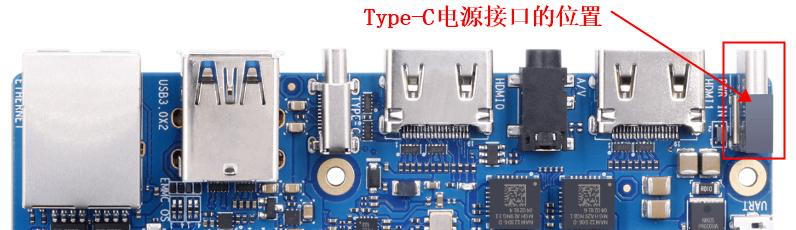
\includegraphics[keepaspectratio,alt={TYPE-C Power}]{cases/img0/typecp.png}}
  \pandocbounded{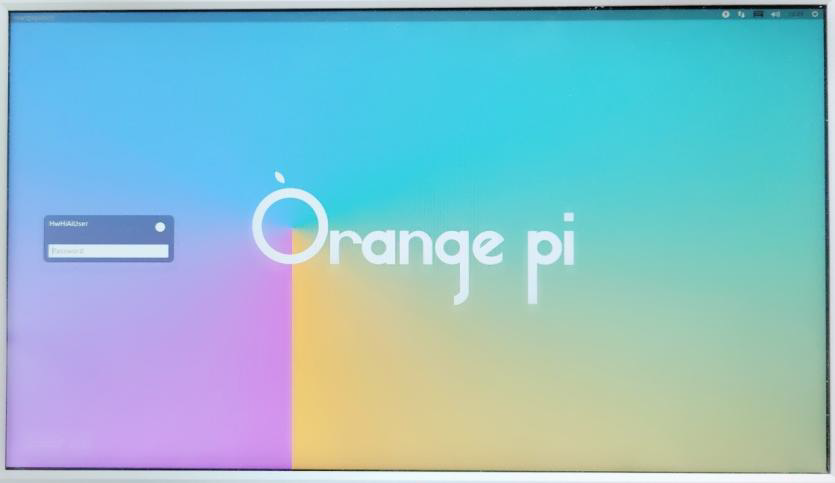
\includegraphics[keepaspectratio,alt={登录}]{cases/img0/beforelogin.png}}
\item
  进入登录界面后,将键盘接入开发板的USB接口中,默认的登录用户名是\passthrough{\lstinline!HwHiAiUser!},输入该账户的密码\passthrough{\lstinline!Mind@123!},登录进入系统。
  \pandocbounded{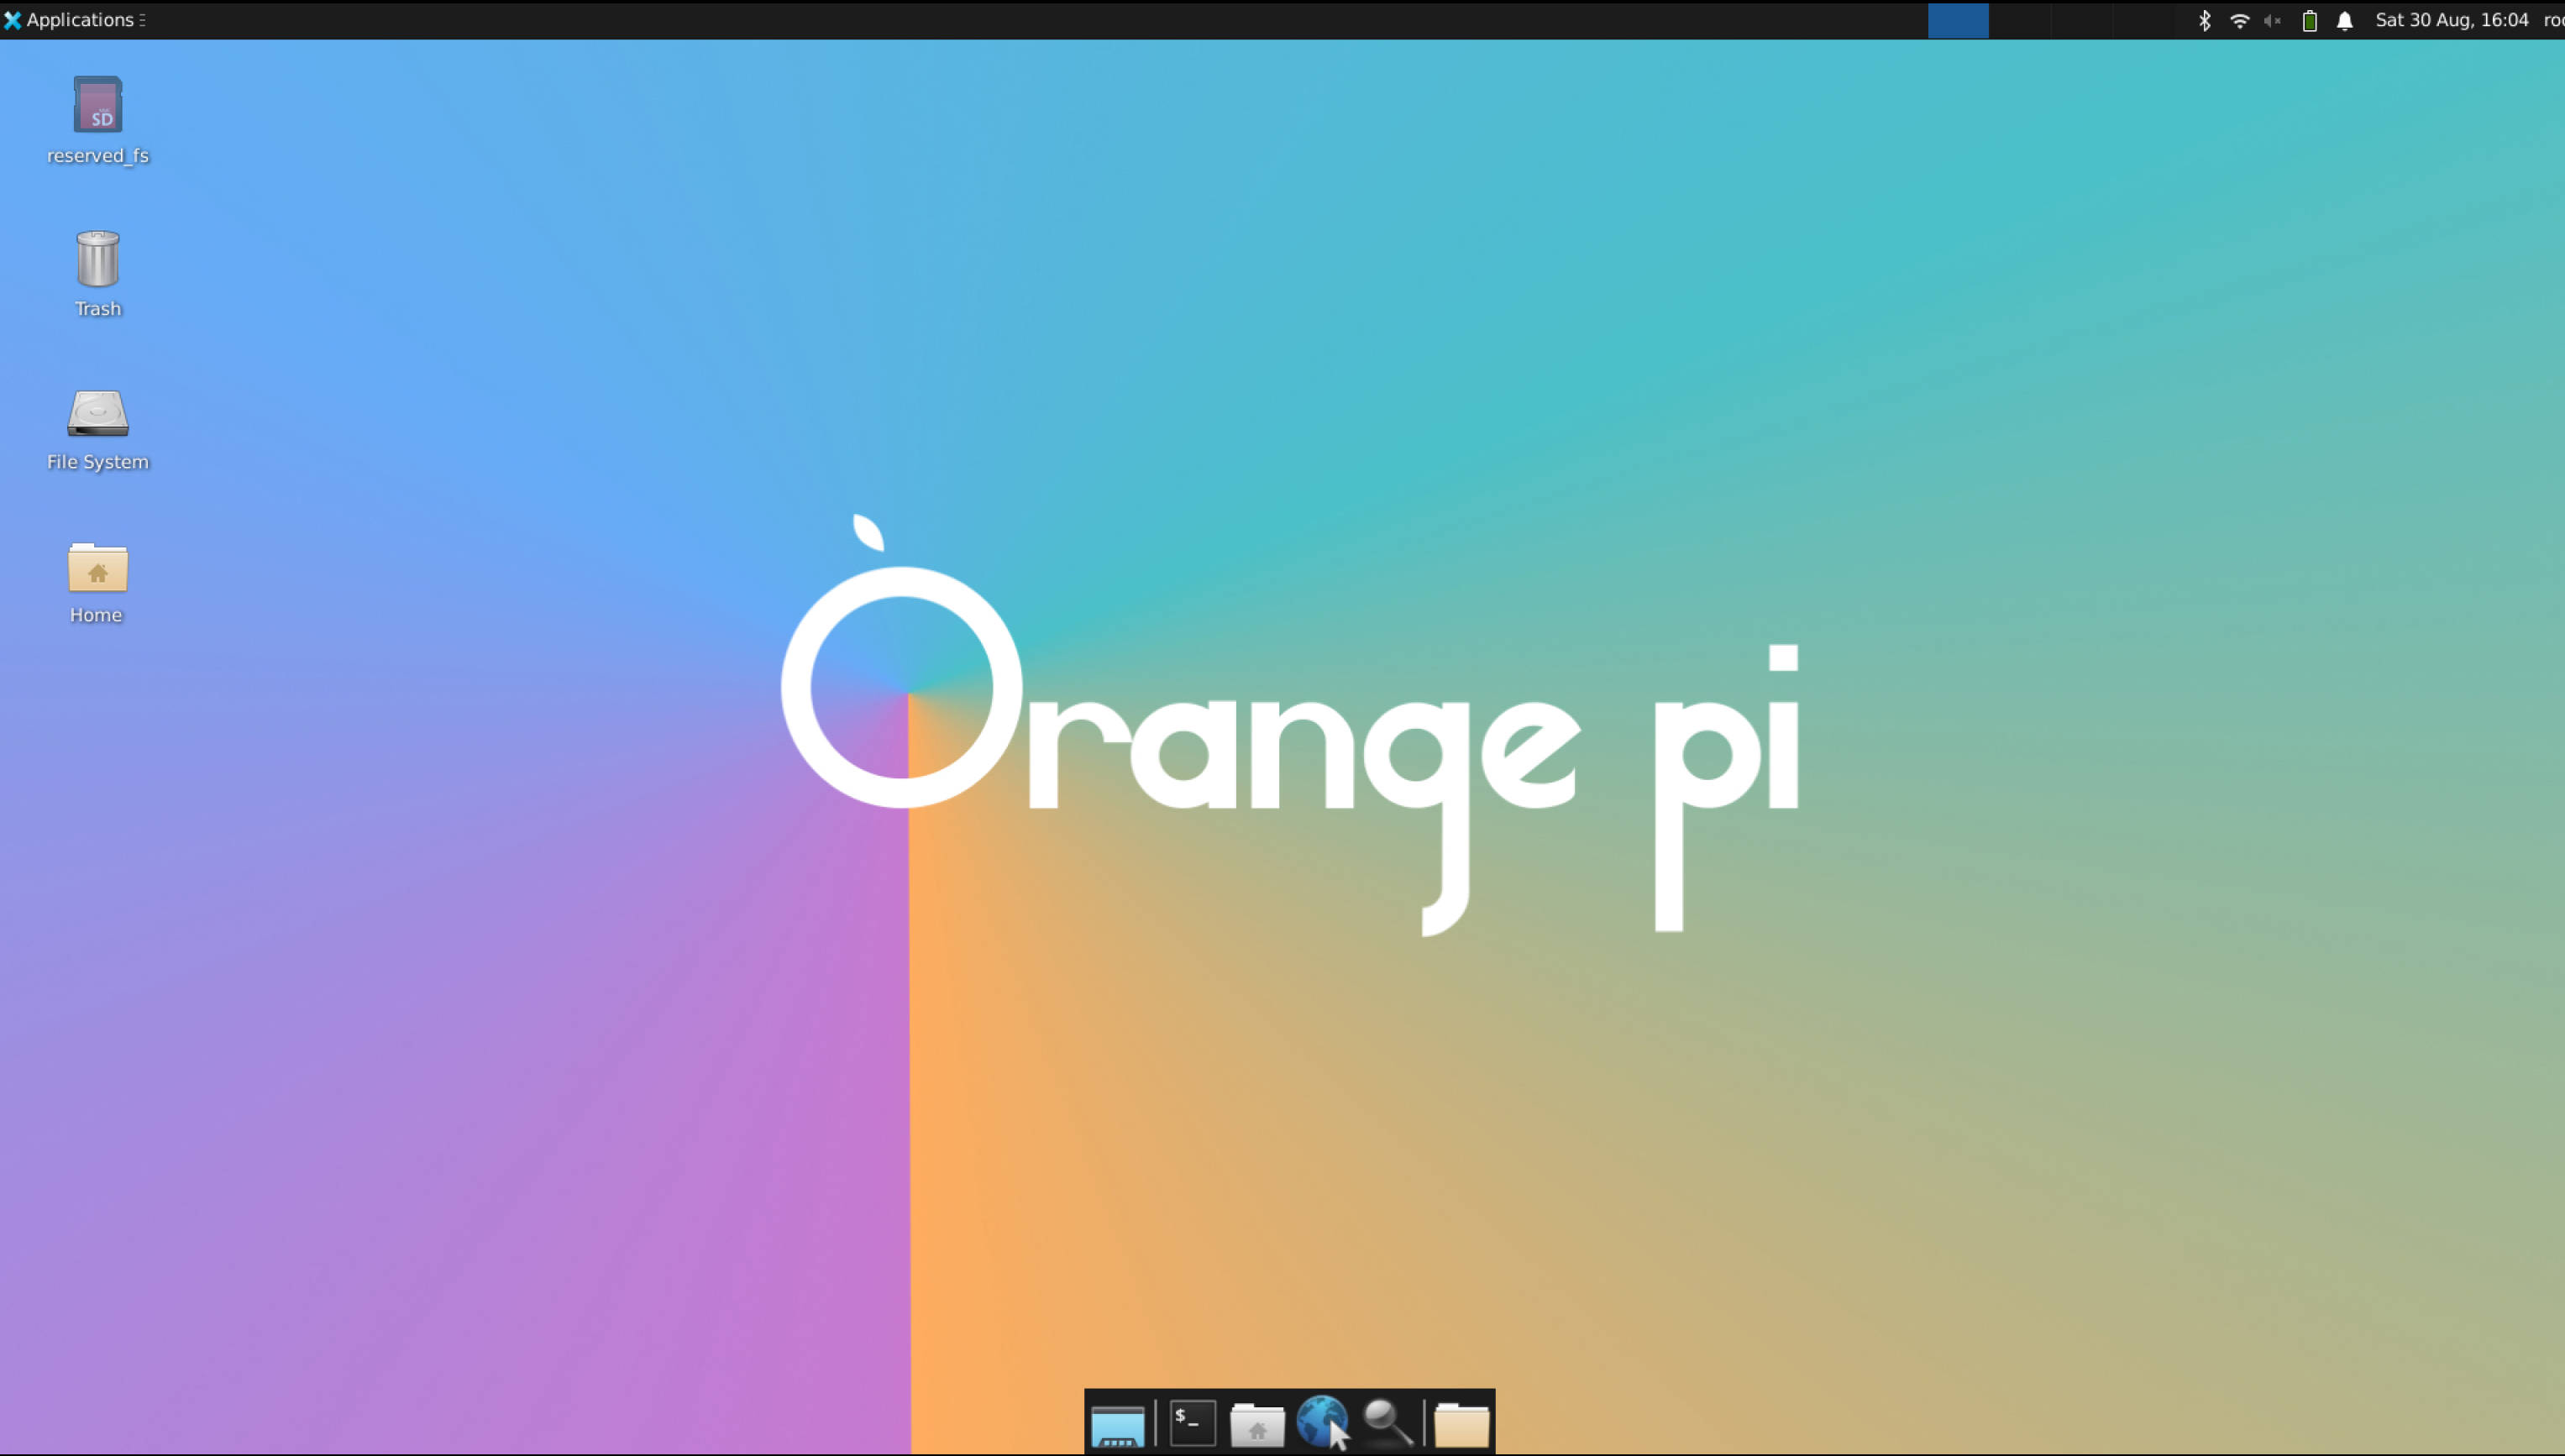
\includegraphics[keepaspectratio,alt={桌面}]{cases/img0/logingui.png}}
  \textgreater{}
  若无法登陆请检查输入的密码是否正确,大小写以及符号是否正确
  默认账户表格: \textbar{} 用户名 \textbar{} 密码 \textbar{} \textbar{}
  :---: \textbar{} :---: \textbar{} \textbar{} root \textbar{} Mind@123
  \textbar{} \textbar{} HwHiAiUser \textbar{} Mind@123 \textbar{}
\end{enumerate}

\begin{itemize}
\tightlist
\item
  串口界面
\end{itemize}

\begin{enumerate}
\def\labelenumi{\arabic{enumi}.}
\tightlist
\item
  使用USB2TTL模块,与开发板的GPIO口进行连线\pandocbounded{\includegraphics[keepaspectratio,alt={开发板串口}]{cases/img0/gpio_ttl.png}},开发板的TX(GPIO8)接入USB2TTL模块的RX接口,开发板的RX(GPIO10)则接入模块的TX接口,并连接好GND接地,在Windows电脑下可以使用PUTTY连接串口。
\item
  使用开发板自带的Micro
  USB接口进行串口调试,该方法更为方便,只需要一根Micro
  USB数据线,接入电脑后打开设备管理器查询对应的串口,然后使用PUTTY进行链接即可。\pandocbounded{\includegraphics[keepaspectratio,alt={MicroUSB串口}]{cases/img0/microusbser.png}}
\end{enumerate}

以Micro USB接口为例: 1. 使用Micro USB数据线连接开发板和电脑 2.
打开电脑的设备管理器,选择端口,寻找开发板对应的串口端口号\pandocbounded{\includegraphics[keepaspectratio,alt={端口号}]{cases/img0/ttl.png}}
3.
打开串口调试软件(PUTTY)\pandocbounded{\includegraphics[keepaspectratio,alt={PUTTY}]{cases/img0/putty.png}},将Connection
Type选择为\passthrough{\lstinline!Serial!},然后在Serial
Line处将端口号修改为设备管理器中查到的端口号,如作者此处端口号为\passthrough{\lstinline!COM3!},此外,还需要将Speed从9600修改为115200,最后点击Open打开串口。
4.
等待出现\passthrough{\lstinline!Ubuntu 22.04.3 LTS orangepiaipro ttyAM0!}字样,输入登录的用户名HwHiAiUser并回车,然后输入密码Mind@123并回车,注意在输入密码的时候屏幕并不会显示任何东西,登陆后的界面如图所示。
\pandocbounded{\includegraphics[keepaspectratio,alt={串口}]{cases/img0/serial.png}}
\pandocbounded{\includegraphics[keepaspectratio,alt={登录成功}]{cases/img0/login.png}}

\subsection{WIFI天线安装指南}\label{wifiux5929ux7ebfux5b89ux88c5ux6307ux5357}

开发版的wifi天线如左侧红色矩形框内所示
\pandocbounded{\includegraphics[keepaspectratio,alt={wifiant}]{cases/img0/wifiant.png}}
将其对准开发版的天线接口安装牢固即可,注意不要将天线贴到开发版的背面,也需要注意天线下方的导电胶布也不要接触开发版,否则有可能导致PCB短路烧坏开发版。

\subsection{Ubuntu
Xfce桌面使用说明}\label{ubuntu-xfceux684cux9762ux4f7fux7528ux8bf4ux660e}

目前系统仅支持Ubuntu 22.04 - Jammy系统,内核版本为Linux 5.10 \#\#\#\#
当前版本适配情况
请详见香橙派官方的用户手册,有部分功能仅支持使用官方程序进行测试,无法直接从系统中调用,在使用过程中需注意这些限制。

\subsubsection{板载LED灯}\label{ux677fux8f7dledux706f}

开发版上有两个绿色的LED灯,一个为电源指示灯,另一个为Linux内核指示灯。
\pandocbounded{\includegraphics[keepaspectratio,alt={电源指示灯}]{cases/img0/powerindicator.png}}
\pandocbounded{\includegraphics[keepaspectratio,alt={内核指示灯}]{cases/img0/linuxindicator.png}}
Linux内核指示灯由GPIO4\_14控制,默认情况下则在Linux启动后该灯就会点亮,如需要修改该灯的点亮条件,需要修改内核DTS文件并重新编译Linux系统。

\subsubsection{有线网络连接}\label{ux6709ux7ebfux7f51ux7edcux8fdeux63a5}

\begin{enumerate}
\def\labelenumi{\arabic{enumi}.}
\tightlist
\item
  将网线一端连接开发版的网口,另一端连接交换机/路由器
\item
  在Ubuntu系统中打开终端(terminal),输入\passthrough{\lstinline!ip a s eth0!},ip地址显示在输出的inet一列
\end{enumerate}

\subsubsection{使用无线网络连接}\label{ux4f7fux7528ux65e0ux7ebfux7f51ux7edcux8fdeux63a5}

\begin{itemize}
\tightlist
\item
  使用nmcli连接,首先\passthrough{\lstinline!nmcli dev wifi!}扫描WIFI,然后使用\passthrough{\lstinline!sudo nmcli dev wifi connect wifi\_name password wifi\_passwd!}(将wifi\_name和wifi\_passwd替换为实际的SSID和密码,不支持中文),连接成功后使用\passthrough{\lstinline!ip a s wlan0!}查看wifi地址。
\item
  使用nmtui连接,在终端输入\passthrough{\lstinline!sudo nmtui!}后即可使用键盘对图形界面进行操作,包括连接网络、断开网络、设置静态IP地址等。
\end{itemize}

\subsection{HDMI口使用}\label{hdmiux53e3ux4f7fux7528}

开发板有两个HDMI2.0接口,目前只有HDMI0支持显示Linux系统的桌面,当Linux系统的桌面系统关闭时,HDMI0和HDMI1还可以用于NVR二次开发场景输出图片。

\subsubsection{使用HDMI VDP模式}\label{ux4f7fux7528hdmi-vdpux6a21ux5f0f}

\begin{enumerate}
\def\labelenumi{\arabic{enumi}.}
\tightlist
\item
  将显示器连接至HDMI0接口,登陆进入系统
\item
  打开终端,输入如下命令:
\end{enumerate}

\begin{lstlisting}[language=bash]
sudo -i
cd /opt/opi_test/hdmi0_pic
./update_dt.sh
\end{lstlisting}

\begin{enumerate}
\def\labelenumi{\arabic{enumi}.}
\setcounter{enumi}{2}
\tightlist
\item
  等待系统重启后,注意此时HDMI接口不会再有输出,使用远程ssh或者串口登陆系统,输入如下命令:
\end{enumerate}

\begin{lstlisting}[language=bash]
sudo -i
cd /opt/opt_test/hdmi0_pic
./test.sh
\end{lstlisting}

可以发现显示屏会输出一张图片,若需要使用hdmi1输出,则只需要将上文的hdmi0修改为hdmi1。

\subsubsection{恢复HDMI DRM模式}\label{ux6062ux590dhdmi-drmux6a21ux5f0f}

进入终端,输入如下命令:

\begin{lstlisting}[language=bash]
sudo -i
cd /opt/opi_test/hdmi_desktop
./update_dt.sh
\end{lstlisting}

等系统重启后即可。

\subsection{USB摄像头使用}\label{usbux6444ux50cfux5934ux4f7fux7528}

将USB摄像头插入开发版的USB3.0接口中,然后输入如下命令查询摄像头:

\begin{lstlisting}[language=bash]
sudo apt-get update
sudo apt-get install -y v4l-utils
sudo v4l2-ctl --list-devices
\end{lstlisting}

接着安装fswebcam\passthrough{\lstinline!sudo apt-get install -y fswebcam!},就可以使用fswebcam进行拍照。

或者使用内置的USBCamera测试代码,运行如下命令,获得一张yuv格式的图片:

\begin{lstlisting}[language=bash]
sudo -i
cd /opt/opi_test/USBCamera
./main /dev/video0
\end{lstlisting}

使用ffplay查看\passthrough{\lstinline!ffplay -pix\_fmt yuyv422 -video\_size 1280*720 out.yuv!}

\subsection{音频使用}\label{ux97f3ux9891ux4f7fux7528}

Linux内核没有适配耳机和HDMI等的ALSA音频驱动,此部分驱动还在开发中,目前只能通过音频样例代码来测试耳机、HDMI的音频播放和板载MIC的录音功能。或者自行购买Linux系统免驱的USB外置声卡,经测试可以正常使用。
若想要使用USB音频,需要将自行准备的USB声卡或者USB接口的耳机连接至USB3.0接口,使用\passthrough{\lstinline!arecord -l!}命令查看录音设备的编号,得到编号后,即可开始测试。

\begin{lstlisting}[language=bash]
sudo -i
cd /opt/opi_test/USBAudio
./main plughw:0 # 录制音频
over # 结束录制
\end{lstlisting}

若需要播放音频,则使用\passthrough{\lstinline!ffplay -ar 44100 -ac 2 -f s16le audio.pcm!}

开发版具有3.5MM的接口,但是如前文所述,目前Linux系统内核并无驱动,使用3.5MM接口播放与录制需要使用指定的测试程序。
播放:

\begin{lstlisting}[language=bash]
sudo -i
cd /opt/opi_test/audio
./sample_audio play 2 qzgy_48k_16_mono_30s.pcm
\end{lstlisting}

录音:

\begin{lstlisting}[language=bash]
sudo -i
cd /opt/opi_test/audio
./sample_audio capture test.pcm # 录音
./sample_audio play 2 test.pcm # 播放
\end{lstlisting}

\subsection{GPIO口的引脚顺序}\label{gpioux53e3ux7684ux5f15ux811aux987aux5e8f}

如图,单号引脚和双号引脚分别在一排。
\pandocbounded{\includegraphics[keepaspectratio,alt={GPIO}]{cases/img0/gpio.png}}
\pandocbounded{\includegraphics[keepaspectratio,alt={GPIO2}]{cases/img0/gpio2.png}}

注意事项: 1.
40pin接口中总共有26个GPIO口,但8号和10号引脚默认是用于调试串口功能的,并且这两个引脚和Micro
USB调试串口是连接在一起的,所以这两个引脚请不要设置为GPIO等功能。 2.
所有的GPIO口的电压都是3.3v。 3.
40pin接口中27号和28号引脚只有I2C的功能,没有GPIO等其他复用功能,另外这两个引脚的电压默认都为1.8v。

\subsubsection{GPIO测试工具}\label{gpioux6d4bux8bd5ux5de5ux5177}

目前开发板的系统镜像已经预装了gpio\_operate工具,该工具可用于设置GPIO管脚的输入与输出方向,也可将每个GPIO管脚独立的设为0或1。
查阅该工具的帮助:

\begin{lstlisting}[language=bash]
sudo -i
gpio_operate -h
\end{lstlisting}

查询GPIO管脚方向
使用\passthrough{\lstinline!gpio\_operate get\_direction gpio\_group gpio\_pin!},其中gpio\_group
是GPIO口对应的分组,取值在{[}0,8{]}之间,gpio\_pin则是GPIO口的管脚号,取值{[}0,31{]}之间,例如GPIO1\_01,获取其方向的代码为\passthrough{\lstinline!gpio\_operate get\_direction 1 01!},得到的结果如图所示,value为0是输入方向,value为1则为输出方向,如此处GPIO1\_01的方向为输入方向。
\pandocbounded{\includegraphics[keepaspectratio,alt={gpio方向}]{cases/img0/gpio_direction.png}}
若需要修改GPIO的管脚方向,则使用另一条命令\passthrough{\lstinline!gpio\_operate set\_direction gpio\_group gpio\_pin direction!},gpio\_group、gpio\_pin和direction的定义与上文一致,只需要根据需要将gpio口修改为需要的方向即可。
另外还能通过这个工具查询和设置GPIO管脚的电平信号,\passthrough{\lstinline!gpio\_operate get\_value gpio\_group gpio\_pin!}用于查询管脚的状态为高电平(1)亦或是低电平(0),如\passthrough{\lstinline!gpio\_operate get\_value 1 01!},得到的value为1,说明是高电平,若value值是0,则说明是低电平。
\pandocbounded{\includegraphics[keepaspectratio,alt={gpio状态}]{cases/img0/gpio_status.png}}
同时,也可以使用\passthrough{\lstinline!gpio\_operate set\_value gpio\_group gpio\_pin value!}来设置默认的管脚电平,注意设置管脚值前,请确保已将GPIO管脚的方向设置为输出!

\subsubsection{SPI测试}\label{spiux6d4bux8bd5}

开发板具有SPI功能,且Ubuntu系统默认配置了SPI的Master功能,SPI总线为SPI0,SDO对应的GPIO为19(GPIO2\_27),SDI对应的GPIO为21(GPIO2\_28),SCLK对应的GPIO为23(GPIO2\_25),CS(片选)对应的GPIO为24(GPIO2\_26)。
查看ubuntu系统中存在的spi设备\passthrough{\lstinline!ls /dev/spidev*!}
\pandocbounded{\includegraphics[keepaspectratio,alt={SPI设备}]{cases/img0/spidevices.png}}

首先测试一下SPI在未连接MISO(SDI)和MOSI(SDO)两个管脚情况下的输出,在终端输入\passthrough{\lstinline!sudo spidev\_test -v -D /dev/spidev0.0!},得到如下结果
\pandocbounded{\includegraphics[keepaspectratio,alt={spidev结果}]{cases/img0/spidev1.png}}
可以发现TX和RX的结果不尽相同,说明此时开发板已经调用SPI接口的驱动在向外发送数据,但是没收到数据,接下来我们使用杜邦线将SDI和SDO连接,构成一个回环,再次运行上述命令,可以发现TX和RX的数据一致,说明SPI的发送和接收功能正常,可以通过spidev命令调用SPI接口了。

\subsubsection{wiringOP}\label{wiringop}

这是一个高性能的GPIO
